%=========================================================
% TRABALHO DE CONCLUSÃO DE CURSO — PROJETO DOMUS
% Faculdade Nova Roma — Ciência da Computação
%
% Documento mestre. As seções estão em sections/. As figuras em figures/.
% Compilar:  pdflatex main.tex   (duas vezes, para sumário/listas/refs)
%   ou:      latexmk -pdf main.tex
%
% Este template reaproveita o formato institucional (extarticle + timbre) e
% traz TODA a estrutura da monografia DOMUS já esqueletada e semeada com o
% conteúdo real do projeto. Preencha os trechos marcados com [...].
%=========================================================
\documentclass[a4paper,12pt]{extarticle}

\usepackage[brazil]{babel}
\usepackage[utf8]{inputenc}
\usepackage[T1]{fontenc}

% Fonte sem serifa (padrão visual do documento institucional)
\usepackage[scaled]{helvet}
\renewcommand{\familydefault}{\sfdefault}

\usepackage{graphicx}
\usepackage{tikz}
\usetikzlibrary{arrows.meta,positioning,shapes.geometric,calc,fit,backgrounds}
\usepackage{eso-pic}
\usepackage[a4paper,top=2.5cm,bottom=2.5cm,left=3cm,right=3cm]{geometry}
\usepackage{booktabs}
\usepackage{longtable}
\usepackage{float}
\usepackage{setspace}
\usepackage{indentfirst}
\usepackage{titlesec}
\usepackage{caption}
\captionsetup{font=small,labelfont=bf}
\usepackage[hidelinks]{hyperref}

\graphicspath{{figures/}}

%--------------------------------------------------------
% Dados do trabalho  (PREENCHA)
%--------------------------------------------------------
\newcommand{\tccautor}{Juliano Freitas}
% Título direcional (contribuição a um objetivo, não resultado alcançado — ver §1).
% Alternativa mais conservadora está comentada abaixo.
\newcommand{\tcctitulo}{DOMUS: uma arquitetura \textit{local-first} de baixo custo para a democratização da automação residencial por voz em português}
% \newcommand{\tcctitulo}{DOMUS: arquitetura local-first de baixo custo para comissionamento e controle de dispositivos Wi-Fi sem dependência permanente de nuvem}
\newcommand{\tccorientador}{Prof.\ MSc.\ Henning Summer}
\newcommand{\tcccoorientador}{}
\newcommand{\tcclocal}{Recife}
\newcommand{\tccano}{2026}

%--------------------------------------------------------
% Formatação de títulos (numerados, negrito; seções em caixa alta)
%--------------------------------------------------------
\titleformat{\section}{\normalfont\bfseries}{\thesection.}{0.5em}{\MakeUppercase}
\titleformat{\subsection}{\normalfont\bfseries}{\thesubsection}{0.5em}{}
\titleformat{\subsubsection}{\normalfont\bfseries\itshape}{\thesubsubsection}{0.5em}{}
\titlespacing*{\section}{0pt}{1.4\baselineskip}{0.7\baselineskip}
\titlespacing*{\subsection}{0pt}{1.1\baselineskip}{0.5\baselineskip}
\titlespacing*{\subsubsection}{0pt}{0.9\baselineskip}{0.4\baselineskip}

\onehalfspacing
\setlength{\parindent}{1.5cm}

%--------------------------------------------------------
% TIMBRE — papel timbrado institucional em todas as páginas
%--------------------------------------------------------
\AddToShipoutPictureBG{%
  \begin{tikzpicture}[remember picture,overlay]
    \node[anchor=north west, inner sep=0, xshift=-10mm, yshift=10mm]
      at (current page.north west) {
\includegraphics{timbre/background-nr.png}};
    \node[anchor=north east, inner sep=1.3cm, yshift=5mm]
      at (current page.north east) {
\includegraphics{timbre/logo-nr.png}};
  \end{tikzpicture}%
}

\begin{document}
\pagenumbering{gobble}

%=================== ELEMENTOS PRÉ-TEXTUAIS ===================
%======================= CAPA =======================
\begingroup
\singlespacing
\begin{center}
\vspace*{0.5cm}
{\bfseries FACULDADE NOVA ROMA}\\[2pt]
{\bfseries CURSO DE CIÊNCIA DA COMPUTAÇÃO}

\vfill

{\bfseries \tccautor}

\vfill

{\large\bfseries \MakeUppercase{\tcctitulo}}

\vfill
\vfill

{\bfseries \MakeUppercase{\tcclocal}}\\[2pt]
{\bfseries \tccano}
\end{center}
\endgroup
\newpage

%======================= FOLHA DE ROSTO =======================
\begingroup
\singlespacing
\begin{center}
\vspace*{1.2cm}

{\bfseries \tccautor}

\vfill

{\large\bfseries \tcctitulo}
\end{center}

\vspace{1.2cm}

% Natureza do trabalho — bloco recuado à direita (padrão ABNT)
\hspace*{7cm}\begin{minipage}{7.5cm}
\singlespacing\small
Trabalho de Conclusão de Curso apresentado como requisito para aprovação na
disciplina de Trabalho de Conclusão de Curso~II do curso de Ciência da
Computação da Faculdade Nova Roma (Caruaru/Recife).

\vspace{0.8cm}
Orientador: \tccorientador
\end{minipage}

\vfill

\begin{center}
{\bfseries \MakeUppercase{\tcclocal}}\\[2pt]
{\bfseries \tccano}
\end{center}
\vspace*{0.6cm}
\endgroup
\newpage

%======================= FOLHA DE APROVAÇÃO =======================
\begingroup
\singlespacing
\begin{center}
\vspace*{1.2cm}
{\bfseries \tccautor}

\vspace{1.0cm}
{\large\bfseries \tcctitulo}
\end{center}

\vspace{1.0cm}
\hspace*{7cm}\begin{minipage}{7.5cm}
\singlespacing\small
Trabalho de Conclusão de Curso apresentado ao curso de Ciência da Computação da
Faculdade Nova Roma como requisito parcial para obtenção do título de Bacharel em
Ciência da Computação.
\end{minipage}

\vspace{1.0cm}
\begin{center}Aprovado em \underline{\hspace{1cm}} de \underline{\hspace{3cm}} de \tccano.\end{center}

\vspace{1.5cm}
\begin{center}
{\bfseries BANCA EXAMINADORA}

\vspace{1.8cm}
\rule{9cm}{0.4pt}\\
\tccorientador\ (Orientador) --- Faculdade Nova Roma

\vspace{1.4cm}
\rule{9cm}{0.4pt}\\
Prof.\ [Membro da Banca 1] --- Faculdade Nova Roma

\vspace{1.4cm}
\rule{9cm}{0.4pt}\\
Prof.\ [Membro da Banca 2] --- Faculdade Nova Roma
\end{center}
\endgroup
\newpage

%======================= RESUMO =======================
\newpage
\begin{center}\textbf{RESUMO}\end{center}
\addcontentsline{toc}{section}{RESUMO}
\vspace{0.4cm}

\noindent
No Brasil, o hardware de automação residencial já é barato --- lâmpadas e tomadas
Wi-Fi genéricas do ecossistema Tuya custam entre R\$~30 e R\$~60 ---, mas transformar
esse hardware em automação utilizável permanece inacessível ao domicílio típico por
três barreiras encadeadas: o custo de \textit{comissionamento} (aplicativos
proprietários, contas em nuvem e portais de desenvolvedor em inglês), a dependência
estrutural de nuvem e os riscos de privacidade. Este trabalho apresenta o DOMUS, uma
prova de conceito de \textit{hub} de automação residencial \textit{local-first},
controlável por voz em português brasileiro processada no próprio \textit{hub}, cuja
tese é que a democratização depende menos do preço do hardware e mais da redução da
barreira de comissionamento (``nuvem uma vez, local para sempre''). O sistema foi
construído com Node.js/NestJS e o padrão \textit{Adapter} para isolar a fragmentação
de protocolos, com reconhecimento de fala por \textit{Whisper} executado no
\textit{hub}. Como resultados, validou-se o controle local do dispositivo TP-Link
Tapo~P110 pelo protocolo KLAP (latências de 201--332~ms) e o \textit{pipeline} de voz
com acurácia de intenção de 87,7\%; custo total, taxa de erro de palavra (WER) e
usabilidade (SUS) são reportados no Capítulo~\ref{cap:resultados}. Conclui-se pela
viabilidade técnica do controle local por voz em português sem dependência permanente
de nuvem; a validação plena da barreira de comissionamento para dispositivos Tuya
permanece como trabalho em andamento.

\vspace{0.5cm}
\noindent\textbf{Palavras-chave:} automação residencial; \textit{local-first};
comissionamento; reconhecimento de voz; privacidade; \textit{Internet of Things}.
\newpage

%======================= ABSTRACT =======================
\newpage
\begin{center}\textbf{ABSTRACT}\end{center}
\addcontentsline{toc}{section}{ABSTRACT}
\vspace{0.4cm}

\noindent
In Brazil, home automation hardware is already cheap --- generic Wi-Fi bulbs and
plugs from the Tuya ecosystem cost between R\$~30 and R\$~60 ---, yet turning that
hardware into usable automation remains out of reach for the typical household due to
three chained barriers: the \textit{commissioning} cost (proprietary apps, cloud
accounts and English-only developer portals), structural cloud dependency, and privacy
risks. This work presents DOMUS, a proof of concept of a \textit{local-first} home
automation hub, controllable by Brazilian Portuguese voice processed on the hub
itself, whose thesis is that democratization depends less on hardware price and more
on lowering the commissioning barrier (``cloud once, local forever''). The system was
built with Node.js/NestJS and the \textit{Adapter} pattern to isolate protocol
fragmentation, with speech recognition via \textit{Whisper} running on the hub. As
results, local control of the TP-Link Tapo~P110 device was validated over the KLAP
protocol (latencies of 201--332~ms) and the voice \textit{pipeline} reached 87.7\%
intent accuracy; total cost, word error rate (WER) and usability (SUS) are reported in
Chapter~\ref{cap:resultados}. We conclude for the technical feasibility of local
Portuguese voice control without permanent cloud dependency; full validation of the
commissioning barrier for Tuya devices remains ongoing work.

\vspace{0.5cm}
\noindent\textbf{Keywords:} home automation; \textit{local-first}; commissioning;
speech recognition; privacy; Internet of Things.
\newpage


\newpage
\listoffigures
\newpage
\listoftables
\newpage
%======================= LISTA DE SIGLAS =======================
\begin{center}\textbf{LISTA DE ABREVIATURAS E SIGLAS}\end{center}
\addcontentsline{toc}{section}{LISTA DE ABREVIATURAS E SIGLAS}
\vspace{0.4cm}

\begingroup
\singlespacing
\setlength{\parindent}{0pt}
\begin{longtable}{@{}p{3.2cm}p{\dimexpr\linewidth-3.4cm}@{}}
API   & \textit{Application Programming Interface} \\
BOM   & \textit{Bill of Materials} (lista de materiais/custos) \\
DPS   & \textit{Data Points} (pontos de dado do protocolo Tuya) \\
HA    & \textit{Home Assistant} \\
IoT   & \textit{Internet of Things} \\
JWT   & \textit{JSON Web Token} \\
KLAP  & \textit{Key Local Authentication Protocol} (TP-Link Tapo) \\
LAN   & \textit{Local Area Network} \\
LGPD  & Lei Geral de Proteção de Dados (Lei n.º 13.709/2018) \\
MVP   & \textit{Minimum Viable Product} \\
PWA   & \textit{Progressive Web App} \\
STT   & \textit{Speech-to-Text} \\
SUS   & \textit{System Usability Scale} \\
TTS   & \textit{Text-to-Speech} \\
WER   & \textit{Word Error Rate} (taxa de erro de palavra) \\
\end{longtable}
\endgroup
\newpage


\newpage
\tableofcontents
\newpage

%=================== ELEMENTOS TEXTUAIS ===================
\pagenumbering{arabic}
%========================================================================
% CAPÍTULO 1 — INTRODUÇÃO
% Incluído por \input em main.tex. NÃO adicionar preâmbulo nem \begin{document}.
% Citações: só o conjunto canônico definido em sections/referencias.tex.
%========================================================================
\section{Introdução}\label{cap:intro}

A automação residencial deixou de ser um artigo de luxo e tornou-se um produto de
prateleira: no Brasil, uma lâmpada ou uma tomada Wi-Fi genérica --- em geral
construídas sobre a plataforma \textit{Tuya} --- custam entre R\$~30 e R\$~60 no
varejo. O mercado nacional de \textit{smart home} foi estimado em cerca de
US\$~2,7~bilhões em 2024, com projeção de crescimento próximo a 10\%~ao~ano até 2033
(IMARC, 2025), e a expansão brasileira, da ordem de 30\%~ao~ano, supera com folga a
média global de aproximadamente 12\%~ao~ano (IDC, 2024). O barateamento do hardware,
portanto, já ocorreu. Ainda assim, transformar esse hardware barato em automação
efetivamente utilizável permanece fora do alcance do domicílio típico brasileiro.

Os indicadores de adoção evidenciam a distância entre a disponibilidade do produto e
seu uso real. A proporção de domicílios brasileiros com ao menos um dispositivo
inteligente passou de 14,3\% em 2022 para 16,4\% em 2024 (IBGE, 2024), patamar muito
inferior aos cerca de 44\% observados nos Estados Unidos e no Reino Unido e à média
mundial de aproximadamente 33\% (STATISTA, 2023). A adoção nacional é, além de baixa,
profundamente desigual: 17,1\% nos domicílios urbanos contra 7,5\% nos rurais, e
19,8\% na região Sul contra 11,2\% no Nordeste (IBGE, 2024). A
Tabela~\ref{tab:penetracao} sintetiza esses recortes.

\begin{table}[H]
\centering
\caption{Penetração de dispositivos residenciais inteligentes: Brasil (recortes) e
referências internacionais.}
\label{tab:penetracao}
\begin{tabular}{@{}lcl@{}}
\toprule
\textbf{Recorte} & \textbf{Penetração (\%)} & \textbf{Fonte} \\
\midrule
Brasil --- domicílios (2022)     & 14,3        & IBGE, 2024 \\
Brasil --- domicílios (2024)     & 16,4        & IBGE, 2024 \\
Brasil --- área urbana           & 17,1        & IBGE, 2024 \\
Brasil --- área rural            & 7,5         & IBGE, 2024 \\
Brasil --- região Sul            & 19,8        & IBGE, 2024 \\
Brasil --- região Nordeste       & 11,2        & IBGE, 2024 \\
Estados Unidos / Reino Unido     & $\approx$44 & STATISTA, 2023 \\
Média mundial                    & $\approx$33 & STATISTA, 2023 \\
\bottomrule
\end{tabular}
\end{table}

Essa desigualdade não se explica por preço de compra, e sim por barreiras que se
acumulam depois da aquisição. A primeira é a conectividade: apenas 22\% dos
domicílios brasileiros dispõem de uma conexão à internet considerada satisfatória,
disparidade que se aprofunda por renda --- 73\% na classe A contra 3\% nas classes
D e~E (CETIC.br, 2024). Como a maioria dos dispositivos comerciais depende de
servidores do fabricante para funcionar, a casa ``inteligente'' deixa de operar
justamente onde a conectividade é mais precária. A segunda é demográfica: o Brasil
envelhece --- a parcela da população com 65 anos ou mais alcançou 10,9\% em 2022
(IBGE, 2024) --- e os idosos, que estão entre os que mais se beneficiariam de
interfaces por voz, são também os menos familiarizados com o letramento digital que a
instalação desses produtos exige. A terceira é a privacidade: o modelo comercial
dominante transmite continuamente áudio e hábitos domésticos a terceiros, o que
tensiona os princípios de minimização e finalidade da Lei Geral de Proteção de Dados
--- LGPD (BRASIL, 2018).

Convém, desde já, delimitar o que \textit{não} é o problema deste trabalho. O custo de
compra do dispositivo é tratado aqui como \textbf{premissa}, e não como a dor a ser
resolvida: o hardware Wi-Fi genérico já é acessível. O obstáculo decisivo à
democratização é outro --- é o \textbf{custo de comissionamento} (a instalação, o
pareamento e a configuração de cada aparelho, que exigem aplicativos proprietários,
criação de contas em nuvem e, para qualquer forma de controle local, o uso de portais
de desenvolvedor em inglês e ferramentas de linha de comando) somado à
\textbf{dependência estrutural de nuvem} para a operação cotidiana. É essa combinação,
e não o preço, que separa o hardware barato da automação utilizável. O princípio
operacional que orienta a proposta resume essa inversão de prioridades: ``nuvem uma
vez, local para sempre''.

\subsection{Problema de pesquisa}

O obstáculo central à democratização da automação residencial no Brasil não é o preço
do hardware --- já acessível ---, mas a \textbf{complexidade de instalar, conectar e
operar} os dispositivos, agravada pela dependência de nuvem e por aplicativos
proprietários. Cada dispositivo, ainda que barato, chega ao usuário atrelado ao
aplicativo e à conta em nuvem de seu fabricante; o controle local, quando existe,
depende de credenciais obtidas em portais de desenvolvedor voltados a especialistas.
O resultado é uma barreira de letramento digital que exclui precisamente os grupos que
mais se beneficiariam da tecnologia --- domicílios de menor renda, populações rurais e
do Nordeste, e a população idosa em crescimento. Formula-se, assim, o problema de
pesquisa: \textit{como tornar a automação residencial acessível a um usuário não
técnico, preservando a privacidade e o funcionamento sem dependência permanente de
nuvem?}

\subsection{Pergunta norteadora e hipótese}

Do problema deriva a seguinte \textbf{pergunta norteadora}: é viável um sistema de
automação residencial funcional, controlável por voz em português brasileiro,
\textit{local-first} e baseado em hardware de baixo custo, que possa ser
\textit{comissionado} por um usuário não técnico sem o aplicativo do fabricante e sem
portais de desenvolvedor?

Diferentemente de uma alegação socioeconômica ampla e não verificável, adota-se aqui
uma \textbf{hipótese de viabilidade falsificável dispositivo a dispositivo}, formulada
de modo a ser confirmada ou refutada por evidência empírica de cada aparelho:

\begin{quote}
\textit{É tecnicamente viável comissionar e controlar localmente, sem aplicativo do
fabricante e sem portais de desenvolvedor, dispositivos Wi-Fi genéricos de baixo
custo, com comandos de voz em português brasileiro processados integralmente no
\textit{hub}, a um custo incremental total inferior a R\$~200.}
\end{quote}

A hipótese é testada em dois dispositivos representativos do varejo brasileiro, com
status distintos: a tomada TP-Link Tapo~P110 --- na qual a forma plena foi
\textbf{confirmada}, com controle local demonstrado pelo protocolo KLAP a latências de
201 a 332~ms usando credenciais de consumidor (não de desenvolvedor) --- e a lâmpada
Intelbras/Tuya EWS~410 --- cujo comissionamento local permanece \textbf{em aberto (em
validação)}. Registre-se, desde a introdução, que a própria dificuldade de comissionar
a lâmpada Tuya, longe de enfraquecer o argumento, constitui \textbf{evidência empírica
da barreira} que este trabalho investiga: se a etapa se mostra custosa até para o
autor, a fortiori o é para o usuário não técnico. Os detalhes dessa evidência são
apresentados no Capítulo~6.

\subsection{Objetivos}

\subsubsection{Objetivo geral}

Demonstrar a viabilidade técnica de um \textit{hub} de automação residencial
\textit{local-first}, de baixo custo e controlável por voz em português brasileiro,
cujo mecanismo de comissionamento reduza a barreira de acesso do usuário não técnico.

\subsubsection{Objetivos específicos}

\begin{enumerate}
  \item Projetar uma arquitetura de software que isole a heterogeneidade de protocolos
        de dispositivos (Tuya, Tapo e outros) atrás de uma interface única, de modo a
        permitir a extensão do sistema sem reescrita do núcleo.
  \item Implementar o reconhecimento de fala em português brasileiro no próprio
        \textit{hub}, sem envio de áudio à nuvem, transcrevendo o comando localmente e
        descartando o áudio após a interpretação.
  \item Validar experimentalmente o controle local de hardware real, medindo latência
        (por percentis) e confiabilidade da comunicação com os dispositivos.
  \item Investigar e caracterizar um mecanismo de comissionamento de dispositivos
        Wi-Fi genéricos que dispense o aplicativo do fabricante e os portais de
        desenvolvedor.
  \item Definir e aplicar um protocolo de avaliação do artefato, contemplando custo
        total (\textit{Bill of Materials} --- BOM), acurácia de voz (taxa de erro de
        palavra --- WER --- e acurácia de intenção), consumo de energia e usabilidade
        junto ao público-alvo (\textit{System Usability Scale} --- SUS).
        % [...] A coletar: BOM datada em 2 cenários (hub reaproveitado × completo);
        % WER sobre corpus pt-BR (>=50 enunciados, >=3 falantes); SUS com n=3-5.
\end{enumerate}

\subsection{Justificativa}

A relevância deste trabalho decorre da convergência entre uma necessidade social e uma
lacuna técnica. Do lado social, os dados apresentados evidenciam uma adoção baixa e
desigual (IBGE, 2024; STATISTA, 2023), condicionada por conectividade precária em boa
parte dos domicílios (CETIC.br, 2024) e por uma transição demográfica que amplia a
população idosa (IBGE, 2024) --- público para o qual a interação por voz representa uma
porta de entrada natural, desde que não exija letramento técnico para a instalação.
Some-se a isso a tensão entre o modelo comercial dependente de nuvem e os princípios da
LGPD (BRASIL, 2018), que torna desejável um arranjo em que os dados domésticos não
saiam da residência.

Do lado técnico, existem soluções maduras de controle local --- notadamente o
\textit{Home Assistant} (HOME ASSISTANT, 2025) --- e um estado da arte de
comissionamento padronizado no protocolo Matter (CONNECTIVITY STANDARDS ALLIANCE,
2024). Contudo, essas soluções ou pressupõem hardware de rádio adicional e ainda caro
ou escasso no varejo popular brasileiro (o caso do Matter), ou, no caso do
\textit{Home Assistant} aplicado ao Wi-Fi barato, pressupõem o \textbf{pareamento
prévio pelo aplicativo do fabricante} --- exatamente a etapa que exclui o usuário não
técnico. A contribuição do DOMUS não está em disputar a sofisticação linguística dos
assistentes comerciais, e sim em atacar o \textbf{comissionamento acessível e local} de
dispositivos Wi-Fi genéricos, alinhado ao paradigma \textit{local-first} descrito por
KLEPPMANN et al. (2019), no qual o usuário é o dono de seus dados e a nuvem é
conveniência, não requisito. A viabilidade do processamento de voz no próprio
\textit{hub}, sem GPU, apoia-se em modelos de reconhecimento de fala robustos como o
\textit{Whisper} (RADFORD et al., 2022), que operam em hardware modesto. O trabalho
adota, ainda, as diretrizes da ABNT para trabalhos acadêmicos (ABNT, 2011) na sua
estruturação e apresentação.

\subsection{Organização do trabalho}

Além desta introdução, o trabalho está organizado em mais seis capítulos. O
\textbf{Capítulo~2 --- Fundamentação teórica} revisa os conceitos de automação
residencial e IoT, a fragmentação de protocolos, o paradigma \textit{local-first}, o
reconhecimento de fala local, a acessibilidade e a segurança e privacidade sob a LGPD.
O \textbf{Capítulo~3 --- Trabalhos relacionados} confronta o DOMUS com os assistentes
comerciais dependentes de nuvem, com o \textit{Home Assistant} e com o protocolo
Matter, delimitando o recorte da contribuição. O \textbf{Capítulo~4 --- Materiais e
métodos} descreve a abordagem metodológica (ciência de projeto e desenvolvimento
orientado a especificações), o padrão \textit{Adapter} como mecanismo contra a
fragmentação, as tecnologias empregadas e os critérios e instrumentos de avaliação. O
\textbf{Capítulo~5 --- Desenvolvimento} detalha a arquitetura e a implementação do
\textit{hub}, do \textit{pipeline} de voz e do mecanismo de comissionamento. O
\textbf{Capítulo~6 --- Resultados e discussão} apresenta as medições obtidas
--- controle local do Tapo~P110, \textit{pipeline} de voz e o estado dos critérios de
sucesso --- e discute seus limites. Por fim, o \textbf{Capítulo~7 --- Considerações
finais} retoma a tese, expõe as limitações e aponta os trabalhos futuros.

%========================= CAPÍTULO 2 =========================
% FUNDAMENTAÇÃO TEÓRICA
% Incluído via \input em main.tex. NÃO reabrir preâmbulo/documento.
% Citações: apenas o conjunto canônico (ver sections/referencias.tex).
% Marcadores [...] indicam dado a coletar; comentários % orientam o preenchimento.
%==============================================================
\section{Fundamentação teórica}\label{cap:fundamentacao}

Este capítulo reúne os conceitos que sustentam o DOMUS e delimita, com precisão,
o problema que o trabalho ataca. Parte-se do panorama de automação residencial e
\textit{Internet of Things} (IoT) no Brasil (Seção~\ref{sec:automacao-iot}) para,
em seguida, fixar o conceito operacional de arquitetura \textit{local-first}
adotado (Seção~\ref{sec:local-first}) e a distinção --- central para a tese ---
entre \textit{comissionar} e \textit{controlar} um dispositivo
(Seção~\ref{sec:comissionamento-controle}). Fecha-se com os fundamentos técnicos
mobilizados na solução: protocolos de dispositivos (Seção~\ref{sec:protocolos}),
reconhecimento de fala (Seção~\ref{sec:fala}), privacidade sob a LGPD
(Seção~\ref{sec:privacidade}) e o padrão de projeto \textit{Adapter}
(Seção~\ref{sec:adapter}).

\subsection{Automação residencial e IoT}\label{sec:automacao-iot}

Automação residencial designa o conjunto de tecnologias que permite monitorar e
controlar, de forma programável, dispositivos de uma residência --- iluminação,
tomadas, sensores e climatização ---, tipicamente integrados por uma rede local e
expostos ao usuário por um aplicativo ou interface de voz. Tais dispositivos são
instâncias domésticas de IoT: objetos físicos dotados de conectividade que trocam
estado e comandos por rede.

O mercado brasileiro de \textit{smart home} está em expansão acelerada, com
projeções de crescimento de dois dígitos ao ano até o início da próxima década
(IMARC, 2025; IDC, 2024; STATISTA, 2023). Ao mesmo tempo, o hardware já é barato:
lâmpadas e tomadas Wi-Fi genéricas do ecossistema Tuya são vendidas por faixas de
poucas dezenas de reais. O gargalo da adoção, portanto, deslocou-se do
\textit{preço do hardware} para as \textit{barreiras de uso}: dependência de
aplicativos proprietários, de contas em nuvem e de certo letramento digital para
concluir a instalação. Esse descompasso é relevante em um país onde o acesso
domiciliar à Internet já é majoritário, mas ainda desigual em qualidade e
autonomia de uso (IBGE, 2024; CETIC.br, 2024).

% AÇÃO DO ALUNO: inserir 1–2 números concretos das fontes acima para ancorar o argumento.
% Ex.: percentual de domicílios com Internet (IBGE/CETIC.br) e tamanho/CAGR do mercado
% brasileiro de smart home (IMARC/IDC/STATISTA). Substituir os [...] abaixo.
Segundo [...], [...\%] dos domicílios brasileiros têm acesso à Internet
(IBGE, 2024), enquanto o mercado nacional de automação residencial é projetado em
[US\$~...] com crescimento anual de [...\%] (IMARC, 2025). O DOMUS parte da
hipótese de que, nesse cenário, a democratização depende menos do custo do
hardware e mais da redução da barreira de instalação.

\subsection{Arquitetura local-first}\label{sec:local-first}

O termo \textit{local-first} foi cunhado por KLEPPMANN et al. (2019) no contexto
de \textit{software colaborativo} (editores de texto, planilhas, quadros). Naquele
sentido, um sistema \textit{local-first} mantém a cópia canônica dos dados no
dispositivo do próprio usuário --- e não em um servidor remoto ---, opera sem
conexão, trata a rede como recurso \textit{opcional} de sincronização e preserva
propriedade, longevidade e privacidade dos dados. Os autores propõem sete ideais e
apoiam a sincronização entre réplicas em estruturas de dados livres de conflito
(\textit{Conflict-free Replicated Data Types}, CRDTs), voltadas a \textit{múltiplos
dispositivos editando o mesmo documento}.

O DOMUS adota o \textit{princípio} de KLEPPMANN et al. (2019) --- ``você é dono dos
seus dados, apesar da nuvem'' ---, mas o \textit{objeto} é distinto: não é um
documento colaborativo, e sim um \textbf{plano de controle} de dispositivos
físicos. Por isso, define-se aqui \textit{local-first} de forma \textbf{operacional}
para este trabalho: o plano de controle do DOMUS --- o reconhecimento de fala
(\textit{Whisper}), os \textit{adapters} de dispositivo, as credenciais/chaves de
controle (\textit{local\_key} do Tuya e a sessão KLAP do Tapo) e os dados de
telemetria e histórico --- \textbf{existe e funciona apenas na instalação local}
(o \textit{hub} na LAN do usuário). A nuvem não é dependência de tempo de execução:
quando muito, é acionada \textit{uma única vez} e de forma \textit{explícita e
comentada} --- por exemplo, para obter a \textit{local\_key} no momento do
comissionamento ---, nunca no laço de controle do dia a dia. Sintetiza-se essa
postura no lema de projeto ``nuvem uma vez, local para sempre''.

Três diferenças em relação à acepção original de KLEPPMANN et al. (2019) merecem
registro. Primeiro, não há problema de \textit{merge} concorrente entre réplicas
(não há CRDTs): o estado canônico do dispositivo é o próprio dispositivo, e o
\textit{hub} é a única autoridade de controle na LAN. Segundo, a preocupação
central desloca-se de \textit{colaboração offline} para \textit{soberania do plano
de controle} --- garantir que o comando de voz e a ação sobre a lâmpada não
dependam de um datacenter. Terceiro, o requisito de privacidade (Seção~\ref{sec:privacidade})
é reforçado pela localidade do processamento de áudio, e não apenas pela posse dos
documentos. Quando o controle local falha, o sistema \textbf{avisa} em vez de cair
silenciosamente para a nuvem --- decisão de projeto que torna a localidade
verificável pelo usuário.

\subsection{Comissionamento versus controle}\label{sec:comissionamento-controle}

A distinção que organiza toda a contribuição deste trabalho é a que separa
\textbf{comissionamento} (\textit{commissioning}) de \textbf{controle}:

\begin{itemize}
  \item \textbf{Controle:} com o dispositivo \textit{já} na Wi-Fi da casa,
        emitir comandos (ligar/desligar, ajustar brilho) e ler estado
        (potência, energia). É o problema ``bem resolvido''.
  \item \textbf{Comissionamento:} levar um dispositivo \textit{de fábrica} a
        entrar na Wi-Fi doméstica \textit{e} receber a credencial que habilita o
        controle local --- idealmente \textbf{sem} o aplicativo do fabricante nem
        conta em nuvem. É o problema em aberto que o DOMUS ataca.
\end{itemize}

Essa fronteira explica por que uma plataforma madura como o Home Assistant (HA)
não dispensa a contribuição do DOMUS. O HA oferece amplitude de \textit{controle}
--- inclusive local, após o \textit{onboarding} --- por meio de suas integrações,
mas as integrações oficiais de Tuya e de TP-Link/Tapo \textbf{pressupõem o
pareamento prévio pelo aplicativo do fabricante} (Smart Life/Tuya, Kasa/Tapo) e uma
conta em nuvem, limitando-se, no caso Tuya, a \textit{recarregar} dispositivos que
já foram pareados por fora (HOME ASSISTANT, 2025). Onde o HA comissiona de fato ---
via Matter ou Improv-over-BLE ---, exige rádio Bluetooth do celular ou
\textit{firmware} aberto embarcado, requisitos que o hardware-alvo de baixo custo
(Seção~\ref{sec:protocolos}) não satisfaz. Ou seja, mesmo o HA \textit{terceiriza o
comissionamento} para o app do fabricante. A análise detalhada dessa dependência,
com as fontes por integração, é desenvolvida no
Capítulo~\ref{cap:trabalhos-relacionados}; aqui basta fixar o conceito: o DOMUS
posiciona sua contribuição exatamente no \textit{gap} de comissionamento
\textit{local-first} que o HA deixa aberto.

\subsection{Protocolos de dispositivos}\label{sec:protocolos}

A automação residencial de baixo custo é marcada por forte heterogeneidade de
protocolos, o que motiva o padrão \textit{Adapter} (Seção~\ref{sec:adapter}).
Quatro famílias são relevantes ao escopo do DOMUS:

\begin{itemize}
  \item \textbf{Wi-Fi genérico Tuya:} ecossistema dominante na faixa mais barata
        do varejo brasileiro (marcas ``white-label'', incluindo a linha Intelbras
        Izy). O controle local usa a \textit{local\_key} por dispositivo, gerada na
        nuvem durante o pareamento; a documentação da plataforma cobre a pilha de
        provisionamento e os \textit{Data Points} (DPS) do protocolo (TUYA, 2025).
        É o caminho de menor custo, porém o de comissionamento mais dependente do
        app proprietário.
  \item \textbf{Wi-Fi Tapo (KLAP):} a TP-Link adota, nos modelos recentes (como a
        tomada Tapo~P110), o protocolo \textit{Key Local Authentication Protocol}
        (KLAP) para autenticação e controle local após o \textit{setup}
        (TP-LINK, 2024). O controle não transita pela nuvem; o \textit{setup}
        inicial, porém, usa BLE proprietário e o app Tapo/Kasa.
  \item \textbf{Zigbee:} rede de malha de baixa potência (IEEE~802.15.4), que exige
        um \textit{coordinator}/\textit{dongle} no \textit{hub}. Reduz dependência
        de Wi-Fi e de nuvem no controle, mas adiciona custo de \textit{gateway} e
        está fora do MVP do DOMUS (fase futura).
  \item \textbf{Matter:} padrão de interoperabilidade mantido pela Connectivity
        Standards Alliance, com comissionamento por credencial aberta
        (CONNECTIVITY STANDARDS ALLIANCE, 2024). É a resposta ``correta'' de longo
        prazo ao problema de comissionamento, mas o hardware Matter ainda é
        \textbf{caro e escasso na faixa de baixo custo no Brasil}, o que o torna
        inviável para o público-alvo deste trabalho no horizonte do MVP.
\end{itemize}

O hardware efetivamente adquirido para validação é a lâmpada Wi-Fi/Tuya Intelbras
EWS~410 e a tomada Wi-Fi/Tapo TP-Link P110 (Tabela~\ref{tab:protocolos}). A
Tabela~\ref{tab:protocolos} contrasta as famílias quanto às duas dimensões que
importam para a tese --- comissionamento e controle local.

\begin{table}[H]
  \centering
  \caption{Protocolos de dispositivos no escopo do DOMUS: comissionamento
           \textit{versus} controle local.}
  \label{tab:protocolos}
  \small
  \begin{tabular}{@{}p{2.6cm}p{2.6cm}p{3.4cm}p{3.4cm}@{}}
    \toprule
    \textbf{Família} & \textbf{Exemplo (alvo)} & \textbf{Comissionamento} &
    \textbf{Controle local} \\
    \midrule
    Wi-Fi Tuya      & Intelbras EWS~410 & App Smart Life + nuvem (barreira central) &
      Sim, via \textit{local\_key} (\texttt{tuyapi}) \\
    Wi-Fi Tapo/KLAP & TP-Link Tapo~P110 & App Tapo/Kasa + BLE no \textit{setup} &
      Sim, sem nuvem (KLAP) \\
    Zigbee          & [modelo a definir] & Emparelhamento por \textit{coordinator} &
      Sim (exige \textit{dongle}); fora do MVP \\
    Matter          & [escasso/caro no BR barato] & Credencial aberta (BLE do
      celular) & Sim, mas hardware inviável no baixo custo \\
    \bottomrule
  \end{tabular}
\end{table}

% AÇÃO DO ALUNO: se desejar, acrescentar coluna de preço (R$) por família a partir da
% BOM real (a coletar) — ver Seção de custos no Capítulo de Resultados.

\subsection{Reconhecimento de fala}\label{sec:fala}

O controle por voz do DOMUS usa reconhecimento automático de fala (\textit{Speech-to-Text},
STT) baseado no modelo \textit{Whisper}, treinado por supervisão fraca em larga
escala e robusto a ruído, sotaques e vocabulário variado (RADFORD et al., 2022).
A decisão de projeto decisiva é \textbf{onde} o modelo executa: no DOMUS, o
\textit{Whisper} roda \textbf{no próprio \textit{hub}} (no \textit{backend}, nunca
no celular), de modo que \textbf{o áudio não é enviado à nuvem}. Essa localidade é o
que torna o reconhecimento de fala coerente com a arquitetura \textit{local-first}
(Seção~\ref{sec:local-first}) e com os requisitos de privacidade
(Seção~\ref{sec:privacidade}): a captura de voz --- dado potencialmente sensível ---
permanece na LAN do usuário.

Como todo modelo de STT, o \textit{Whisper} está sujeito a erros e a
\textbf{alucinações} em trechos de baixa razão sinal-ruído: em execução real do
DOMUS observou-se, por exemplo, a transcrição espúria ``[Som de futebol]'' em
segmentos sem fala. O tratamento adotado (limiar de confiança, segmentação e
\textit{parsing} de intenção tolerante) e a análise quantitativa --- acurácia de
intenção de 87,7\% sobre 138 comandos reais, com a taxa de erro de palavra (WER)
ainda [a coletar] --- são reportados no
Capítulo~\ref{cap:resultados}. Antecipa-se apenas um achado metodologicamente
importante: a acurácia do \textit{reconhecimento/parsing} e o \textit{sucesso de
execução} são métricas distintas, pois a segunda é dominada por falhas de hardware
(dispositivo \textit{offline}, \textit{timeout}), não pelo modelo de fala.

\subsection{Privacidade e LGPD}\label{sec:privacidade}

A Lei Geral de Proteção de Dados Pessoais (LGPD, Lei n.º~13.709/2018) rege o
tratamento de dados pessoais no Brasil e estabelece princípios de finalidade,
necessidade, transparência e segurança, além de fundamentos legais para o
tratamento (BRASIL, 2018). Uma casa automatizada por voz produz dados
particularmente sensíveis: gravações de áudio, padrões de presença e rotina
inferíveis do histórico de acionamentos e do consumo de energia.

A arquitetura \textit{local-first} do DOMUS funciona como \textbf{medida técnica de
privacidade por concepção} alinhada à LGPD: ao processar o áudio no \textit{hub} e
manter dados e credenciais na instalação local (Seção~\ref{sec:local-first}),
minimiza-se a coleta e a transferência de dados pessoais a terceiros --- em contraste
com arquiteturas centradas em nuvem, nas quais áudio e telemetria trafegam para
servidores do fabricante. Em nível de implementação, o projeto adota o princípio de
que segredos nunca são armazenados em texto puro (a \textit{local\_key} do Tuya é
cifrada em repouso) e de que dados são escopados por usuário. O mapeamento formal
dos dados pessoais tratados, das bases legais aplicáveis e das medidas de segurança
--- na forma de [tabela/relatório de conformidade] --- é [a coletar].

% AÇÃO DO ALUNO: inserir tabela (dado pessoal × finalidade × base legal LGPD × medida de
% segurança) e, se aplicável, referência a princípio de privacy-by-design.

\subsection{Padrão Adapter}\label{sec:adapter}

A heterogeneidade de protocolos descrita na Seção~\ref{sec:protocolos} ---
\textit{local\_key}/DPS no Tuya, sessão KLAP no Tapo, malha no Zigbee ---
fragmenta as APIs de controle e ameaça acoplar o núcleo do sistema a bibliotecas
específicas e voláteis. O padrão de projeto \textbf{\textit{Adapter}} resolve esse
problema ao converter a interface de cada dispositivo/biblioteca (por exemplo,
\texttt{tuyapi} e \texttt{tp-link-tapo-connect}) em uma interface comum e estável ---
no DOMUS, a interface \texttt{DeviceAdapter} --- consumida uniformemente pelos
serviços do \textit{hub}. Assim, nenhum \textit{controller} ou serviço invoca uma
biblioteca de IoT diretamente: toda a variabilidade de protocolo fica encapsulada
atrás do \textit{adapter}, e um \texttt{MockAdapter} permite executar e testar o
sistema inteiro sem hardware físico.

Essa escolha tem \textit{prior art} explícito: o modelo de ``integrações'' do Home
Assistant --- cada protocolo isolado atrás de uma interface comum, com fluxo de
configuração próprio --- valida o \textit{adapter pattern} como forma consolidada de
absorver a fragmentação de protocolos em automação residencial (HOME ASSISTANT, 2025).
O DOMUS reusa esse padrão de arquitetura na camada de \textit{controle} e concentra
sua contribuição na camada de \textit{comissionamento} (Seção~\ref{sec:comissionamento-controle}).
A instanciação concreta da interface \texttt{DeviceAdapter} e de seus
\textit{adapters} é detalhada no Capítulo~\ref{cap:desenvolvimento}.

%=========================================================
% CAPÍTULO 3 — TRABALHOS RELACIONADOS
% Incluído via \input em main.tex. NÃO reabrir preâmbulo.
%=========================================================
\section{Trabalhos relacionados}\label{cap:relacionados}

O problema de automação residencial de baixo custo não é novo, e existe um
ecossistema maduro de plataformas que se propõem a controlar dispositivos
heterogêneos a partir de uma interface única. Para posicionar corretamente a
contribuição do DOMUS, é preciso separar duas operações que a literatura de
mercado costuma tratar como uma só: o \textit{controle} (o dispositivo já está na
rede Wi-Fi e recebe comandos de liga/desliga, brilho ou leitura de estado) e o
\textit{comissionamento} (\textit{commissioning}) --- levar um dispositivo de
fábrica para dentro da rede Wi-Fi e obter uma credencial de controle, idealmente
\textbf{sem} o aplicativo do fabricante. As plataformas discutidas a seguir são
fortes na primeira operação e, em regra, terceirizam a segunda para o app
proprietário. É exatamente nessa fronteira que o DOMUS se insere.

\subsection{Home Assistant}\label{sec:home-assistant}

O Home Assistant (HOME ASSISTANT, 2025) é a referência de código aberto para
controle local: sua arquitetura de \textit{integrations} isola cada protocolo
atrás de uma interface comum, com um \textit{config flow} declarativo, e sua
\textit{WebSocket API} oferece um canal de tempo real maduro (\texttt{subscribe\_events},
\texttt{call\_service}, \texttt{get\_states}). Esse desenho valida, como \textit{prior
art}, o \textit{adapter pattern} adotado pelo DOMUS e o canal Socket.IO do seu PWA.

A limitação decisiva, porém, aparece no comissionamento. Para o hardware-alvo
deste trabalho --- lâmpada Tuya/Intelbras EWS 410 e tomada TP-Link Tapo P110 ---
as próprias integrações oficiais do Home Assistant \textbf{pressupõem o aplicativo
do fabricante}. A integração Tuya exige que o dispositivo já tenha sido adicionado
à conta na nuvem por meio do app Smart Life/Tuya Smart antes de qualquer
recarga no hub; a integração TP-Link trata o provisionamento Wi-Fi como
pré-requisito externo, feito no app Kasa/Tapo ou por uma ferramenta de linha de
comando documentada como instável para os modelos Tapo recentes. Os caminhos em
que o Home Assistant de fato comissiona de forma nativa --- Matter e Improv via
BLE --- são \textit{gated} por firmware e por padrões abertos que nem a EWS 410 nem
a Tapo P110 implementam. O gap ``dispositivo de fábrica $\rightarrow$ Wi-Fi $+$
credencial local'' permanece, portanto, aberto.

Disso decorre a decisão de arquitetura registrada no projeto (ADR-001): adotar o
Home Assistant como \textbf{núcleo} de execução inverteria a tese --- ele passaria
a ser a contribuição, e o DOMUS, uma casca de interface --- e, ainda assim,
\textbf{não} resolveria o problema-alvo, porque o comissionamento continuaria
delegado ao app do fabricante. O DOMUS toma emprestado do Home Assistant o modelo
de \textit{adapter}/integração e o design de API em tempo real, mas mantém seu
próprio hub como núcleo; o Home Assistant, se integrado no futuro, entraria como
\emph{uma fonte a mais} sob o \textit{adapter pattern} do DOMUS, de forma coerente
com o padrão, e nunca como orquestrador de \textit{runtime}.

\subsection{OpenHAB}\label{sec:openhab}

O OpenHAB, plataforma de automação em Java com motor de regras e execução local,
compartilha a filosofia \textit{local-first} do Home Assistant e reforça o mesmo
diagnóstico: seus \textit{bindings} cobrem amplamente o \textbf{controle} de
dispositivos já pareados, mas o comissionamento de hardware Wi-Fi proprietário
continua dependente do app do fabricante ou de credenciais obtidas na nuvem do
fornecedor. Sua curva de configuração --- arquivos de \textit{items}, \textit{things}
e \textit{sitemaps} --- também eleva a barreira técnica para o usuário leigo, o
público que o DOMUS pretende atender.
% "..." Se desejar citação formal do OpenHAB, acrescentar a entrada correspondente
% em sections/referencias.tex (fora do conjunto canônico atual) e referenciá-la aqui.

\subsection{Ecossistemas comerciais (Amazon Alexa e Google Home)}\label{sec:comerciais}

Os assistentes comerciais --- Amazon Alexa e Google Home/Assistant --- entregam a
melhor experiência de comissionamento guiado e reconhecimento de voz em português
do mercado, e sustentam a maior fatia de adoção de dispositivos de casa inteligente
(IDC, 2024; STATISTA, 2023), inclusive no cenário brasileiro em expansão
(IMARC, 2025). Essa conveniência, porém, tem dois custos estruturais que colidem
com os princípios deste trabalho. O primeiro é a \textbf{dependência de nuvem}: o
reconhecimento de fala e boa parte da lógica de automação rodam em servidores do
fornecedor, de modo que a queda da internet degrada ou inutiliza o controle, e o
áudio doméstico trafega para fora da residência --- tensão direta com a
minimização de dados prevista na LGPD (BRASIL, 2018). O segundo é o
\textbf{aprisionamento} (\textit{vendor lock-in}): dispositivos, rotinas e a
própria conta ficam atados a um ecossistema proprietário, contrariando o princípio
\textit{local-first}, no qual o usuário mantém a posse e o controle dos próprios
dados a despeito da nuvem (KLEPPMANN et al., 2019). O DOMUS busca a mesma
conveniência de voz \textbf{sem} exportar o áudio nem a lógica de decisão: o
reconhecimento de fala ocorre no próprio hub, com o modelo Whisper
(RADFORD et al., 2022), e não no celular nem na nuvem.

\subsection{Matter}\label{sec:matter}

O padrão Matter (CONNECTIVITY STANDARDS ALLIANCE, 2024) é a resposta da indústria
ao problema de interoperabilidade e comissionamento: define um provisionamento
unificado, via BLE e código QR, entre fabricantes distintos. É, conceitualmente, a
solução mais elegante para o gap aqui discutido. Na prática, contudo, ainda é uma
padronização \textbf{cara e de adoção incipiente} para o público-alvo: exige
hardware certificado, frequentemente um \textit{Thread Border Router} adicional, e
não abrange o parque de dispositivos Wi-Fi de baixo custo já em circulação. O
hardware efetivamente adquirido para este trabalho é ilustrativo: nem a lâmpada
Tuya/Intelbras EWS 410 (TUYA, 2025) nem a tomada TP-Link Tapo P110 (TP-LINK, 2024)
implementam Matter, de modo que nenhum caminho de comissionamento padronizado as
alcança. Matter aponta o futuro desejável da interoperabilidade, mas não resolve o
presente de baixo custo que o DOMUS tem por alvo.

\subsection{Posicionamento do DOMUS}\label{sec:posicionamento}

À luz do exposto, a contribuição do DOMUS não é ``mais uma plataforma de
controle'': é o \textbf{comissionamento acessível e local} de dispositivos Wi-Fi
de fábrica, combinado a \textbf{voz em português brasileiro processada no próprio
hub}, sem dependência permanente de nuvem e a custo compatível com a realidade
brasileira. Nenhuma das soluções analisadas ocupa simultaneamente esses quatro
pontos: o Home Assistant e o OpenHAB são locais mas delegam o comissionamento; os
ecossistemas comerciais oferecem voz e comissionamento guiado mas dependem da
nuvem e aprisionam o usuário; o Matter padroniza mas exige hardware que o
público-alvo não possui. A Tabela~\ref{tab:comparativo} sintetiza esse contraste.

\begin{table}[H]
\centering
\caption{Comparativo entre soluções de automação residencial e o DOMUS.}
\label{tab:comparativo}
\begin{tabular}{@{}lcccc@{}}
\toprule
\textbf{Solução} & \textbf{Controle} & \textbf{Comission.} & \textbf{Voz pt-BR} & \textbf{Baixo} \\
                 & \textbf{local}    & \textbf{sem app/portal} & \textbf{local} & \textbf{custo} \\
\midrule
Home Assistant          & Sim     & Não     & Parcial\textsuperscript{a} & Parcial \\
OpenHAB                 & Sim     & Não     & Parcial\textsuperscript{a} & Parcial \\
Alexa / Google Home     & Não     & Parcial\textsuperscript{b} & Não\textsuperscript{c} & Parcial \\
Matter                  & Sim     & Sim     & N/A\textsuperscript{d}     & Não \\
\textbf{DOMUS}          & \textbf{Sim} & \textbf{Sim}\textsuperscript{e} & \textbf{Sim} & \textbf{Sim}\textsuperscript{f} \\
\bottomrule
\end{tabular}

\vspace{0.3em}
{\footnotesize
\begin{flushleft}
\textsuperscript{a} Requer \textit{add-ons} ou STT externo/nuvem para voz.
\textsuperscript{b} Comissionamento guiado, porém atrelado a conta na nuvem.
\textsuperscript{c} Voz em pt-BR existe, mas é processada na nuvem, não localmente.
\textsuperscript{d} Depende do controlador Matter adotado.
\textsuperscript{e} Objetivo central do trabalho, em validação empírica (ver abaixo).
\textsuperscript{f} Meta $<$ R\$~200 em hardware; BOM detalhado \textit{a coletar}.
\end{flushleft}}
\end{table}

Cabe registrar, com honestidade metodológica, o estágio de validação de cada
frente do DOMUS. No \textbf{controle local}, os resultados já são positivos: a
tomada Tapo P110, acionada localmente pelo protocolo KLAP, respondeu com latências
entre 201 e 332~ms, sem passar pela nuvem TP-Link. Na \textbf{voz}, a interpretação
de intenção atingiu 87,7\% de acurácia sobre 138 comandos reais em português,
com latência mediana (p50) de 463~ms e p95 de 2140~ms; o sucesso de
\textbf{execução} ficou em 66,7\%, dominado por falhas de \textit{hardware offline}
--- e não pelo analisador de comandos ---, com um \textit{outlier} máximo de 12,3~s
correspondente a \textit{timeout} de dispositivo. Registraram-se ainda alucinações
pontuais do Whisper (por exemplo, a transcrição espúria ``[Som de futebol]''),
comportamento conhecido do modelo em trechos de baixa energia acústica.

No \textbf{comissionamento}, a evidência é, por ora, a da própria barreira: o
pareamento da lâmpada Tuya EWS 410 sem o app SmartLife encontra-se
\textbf{bloqueado} e segue em validação --- resultado que, longe de enfraquecer a
tese, confirma empiricamente que o gap atacado é real e não trivialmente
solucionável pelas plataformas existentes. As métricas de qualidade de transcrição
(WER), usabilidade (SUS) e custo consolidado de materiais (BOM) permanecem
\textit{a coletar} [...] e serão reportadas no Capítulo de resultados.
% "..." Inserir, quando disponíveis: WER da transcrição, escore SUS do estudo de
% usabilidade e a lista de materiais (BOM) com o custo total do hardware.

%======================= MATERIAIS E MÉTODOS =======================
% Capítulo 4 — descreve a classificação metodológica, o hardware-alvo, a stack
% de ferramentas e, sobretudo, o PROTOCOLO DE AVALIAÇÃO (quatro métricas
% separadas + SUS + energia + BOM). Os resultados numéricos consolidados vão no
% Capítulo \ref{cap:resultados}; aqui citam-se apenas os valores de um piloto
% que JUSTIFICAM as escolhas de instrumentação.
\section{Materiais e métodos}\label{cap:metodos}

Este capítulo descreve como a prova de conceito (PoC) do DOMUS foi construída e,
principalmente, como ela é avaliada. A ênfase recai sobre o protocolo de avaliação:
para um trabalho cuja tese é que a democratização da automação residencial depende
mais da redução da barreira de comissionamento do que do preço do hardware, é o
método de medição --- e não a mera demonstração de funcionamento --- que sustenta ou
refuta a hipótese. A apresentação segue a NBR~14724 (ABNT, 2011) quanto à estrutura
do trabalho acadêmico.

\subsection{Classificação da pesquisa}\label{sec:classificacao}

Quanto à natureza, esta é uma \textbf{pesquisa aplicada}: parte de um problema concreto
--- famílias brasileiras que possuem hardware barato de automação, mas não conseguem
transformá-lo em automação utilizável --- e produz um artefato que endereça esse
problema. Quanto ao objetivo, caracteriza-se como \textbf{desenvolvimento de uma prova
de conceito (PoC)}: o produto é um sistema executável, o \textit{hub} DOMUS, cuja função
é evidenciar a viabilidade técnica do controle local por voz em português sem
dependência permanente de nuvem, e não um produto comercial acabado.

Metodologicamente, o desenvolvimento é \textbf{orientado a especificações}: cada
integração de dispositivo parte da leitura da documentação e do protocolo real do
fabricante (TP-LINK, 2024; TUYA, 2025) antes da escrita de código, evitando suposições
sobre APIs de IoT que mudam entre versões. Como estratégia central de projeto contra a
\textbf{fragmentação de protocolos} --- cada fabricante expõe um protocolo, um formato de
autenticação e um vocabulário de comandos distintos ---, adota-se o \textbf{padrão de
projeto \textit{Adapter}}. Nenhum controlador ou serviço de aplicação invoca as
bibliotecas de IoT diretamente; toda comunicação atravessa uma interface única
(\texttt{DeviceAdapter}), de modo que a heterogeneidade de Tuya e Tapo fique confinada a
implementações concretas e intercambiáveis. Essa decisão também viabiliza o \textbf{modo
MOCK}, no qual o sistema inteiro executa sem hardware físico, requisito para testes
automatizados reprodutíveis e para a integração contínua.

\subsection{Hardware-alvo}\label{sec:hardware}

O hardware-alvo foi selecionado para ser representativo do que uma família brasileira
compra em varejo popular: dispositivos Wi-Fi de 2,4~GHz, sem \textit{hub} proprietário
dedicado, de dois ecossistemas dominantes e de protocolos deliberadamente distintos, a
fim de exercitar o padrão \textit{Adapter} sob fragmentação real. A lâmpada Intelbras
pertence à linha Izy, que é \textit{white-label} do ecossistema Tuya e, portanto,
coberta pela mesma pilha de protocolo (TUYA, 2025); a tomada TP-Link Tapo utiliza o
protocolo proprietário KLAP (\textit{Key Local Authentication Protocol}). A
Tabela~\ref{tab:hardware} resume os dispositivos e a meta de custo total do arranjo,
fixada em menos de R\$~200 em hardware.

\begin{table}[H]
\centering
\caption{Hardware-alvo da prova de conceito e capacidades expostas.}
\label{tab:hardware}
\small
\begin{tabular}{@{}p{2.9cm}p{2.4cm}p{2.6cm}p{4.0cm}@{}}
\toprule
\textbf{Dispositivo} & \textbf{Modelo} & \textbf{Interface / protocolo} & \textbf{Capacidades expostas} \\
\midrule
Lâmpada LED & Intelbras EWS~410 & Wi-Fi 2,4~GHz / Tuya & liga/desliga, brilho, cor RGB \\
Tomada inteligente & TP-Link Tapo~P110 & Wi-Fi 2,4~GHz / KLAP & liga/desliga, medição de energia (W, kWh) \\
\midrule
\multicolumn{4}{@{}l}{\textit{Meta de custo do arranjo: total de hardware $<$ R\$~200,00 (verificado na BOM datada, Tab.~\ref{tab:bom-proto}).}} \\
\bottomrule
\end{tabular}
\end{table}

A escolha desses dois dispositivos não é arbitrária quanto à validação da tese. A tomada
Tapo~P110 permite exercitar o \textbf{caminho feliz} do controle local: seu protocolo
KLAP é acessível na LAN após uma autenticação local, e a medição de energia fornece um
sinal físico verificável de que um comando surtiu efeito. Já a lâmpada EWS~410 expõe a
\textbf{barreira de comissionamento} sob estudo: o pareamento inicial exige uma conta em
aplicativo proprietário e a obtenção de uma chave local (\texttt{local\_key}) via nuvem,
etapa que se mostrou, empiricamente, um ponto de bloqueio (Seção~\ref{sec:ambiente}).

\subsection{Ferramentas e tecnologias}\label{sec:ferramentas}

O \textit{hub} DOMUS é implementado em \textbf{Node.js~20~LTS} com \textbf{TypeScript} e
o \textit{framework} \textbf{NestJS}, cuja arquitetura modular por injeção de dependência
favorece o isolamento dos \textit{adapters}. A persistência usa \textbf{Prisma} sobre
\textbf{PostgreSQL}, e a comunicação em tempo real entre \textit{hub} e clientes usa
\textbf{Socket.IO} (WebSocket), de modo que mudanças de estado dos dispositivos sejam
refletidas na interface sem \textit{polling}. A interface de usuário é um
\textbf{\textit{Progressive Web App} (PWA)} construído em \textbf{Next.js~15} com
React~19, instalável no celular (\textit{Add to Home Screen}), o que dispensa publicação
em lojas de aplicativos e reforça a proposta \textit{local-first} (KLEPPMANN \textit{et
al.}, 2019).

O reconhecimento de fala (\textit{Speech-to-Text}, STT) usa o modelo \textbf{Whisper}
(RADFORD \textit{et al.}, 2022) executado \textbf{no próprio \textit{hub}} --- nunca no
celular e nunca na nuvem ---, decisão que é ao mesmo tempo de desempenho e de
privacidade. A integração com os dispositivos usa as bibliotecas \textbf{\texttt{tuyapi}}
(ecossistema Tuya/Intelbras) e \textbf{\texttt{tp-link-tapo-connect}} (Tapo), ambas
encapsuladas atrás da interface \texttt{DeviceAdapter}. A Tabela~\ref{tab:stack} consolida
as tecnologias por camada e sua função na PoC.

\begin{table}[H]
\centering
\caption{Ferramentas e tecnologias por camada.}
\label{tab:stack}
\small
\begin{tabular}{@{}p{3.0cm}p{5.0cm}p{4.2cm}@{}}
\toprule
\textbf{Camada} & \textbf{Tecnologia} & \textbf{Função na PoC} \\
\midrule
\textit{Hub}/backend & Node.js~20, TypeScript, NestJS & orquestração, regras, API \\
Persistência & Prisma + PostgreSQL & dispositivos, comandos, energia \\
Tempo real & Socket.IO (WebSocket) & estado ao vivo na interface \\
Interface & Next.js~15 + React~19 (PWA) & \textit{dashboard}, rotinas, voz \\
Voz (STT) & Whisper (no \textit{hub}) & transcrição de comandos pt-BR \\
IoT (\textit{adapters}) & \texttt{tuyapi}, \texttt{tp-link-tapo-connect} & controle local de Tuya e Tapo \\
\bottomrule
\end{tabular}
\end{table}

% Versões exatas conferem com apps/api/package.json: NestJS 11, Prisma 6,
% socket.io 4.8, tuyapi 7.7, tp-link-tapo-connect 2.0.15, nodejs-whisper 0.3.

\subsection{Protocolo de avaliação}\label{sec:protocolo}

A avaliação separa deliberadamente aquilo que a literatura de assistentes de voz
frequentemente confunde num único número. Uma única ``taxa de acerto'' agregada esconde
onde uma cadeia voz~$\rightarrow$~ação falha: se o erro está na transcrição, na
interpretação da intenção ou na execução física no dispositivo. Por isso, definem-se
\textbf{quatro métricas independentes} e três instrumentos complementares (SUS, energia e
BOM). A necessidade dessa separação é empiricamente motivada: em uma execução-piloto com
138 comandos reais, a acurácia de \emph{intenção} foi de 87,7\%, enquanto o sucesso de
\emph{execução} ponta-a-ponta foi de apenas 66,7\% --- diferença dominada por hardware
\textit{offline} no momento do comando, e não por falha do interpretador. Medir os dois
como um só número teria atribuído ao \textit{software} de linguagem uma falha que é do
dispositivo.

\subsubsection{Métrica 1 --- WER (taxa de erro de palavra)}

Avalia isoladamente a camada de transcrição do Whisper. Calcula-se a
\textit{Word Error Rate} pela razão entre edições e o total de palavras de referência:
\[
\mathrm{WER} = \frac{S + D + I}{N},
\]
em que $S$, $D$ e $I$ são, respectivamente, substituições, remoções e inserções em
relação à transcrição de referência, e $N$ é o número de palavras da referência. O
\textbf{corpus de avaliação} conterá \textbf{no mínimo 50 enunciados} de comando,
gravados por \textbf{ao menos 3 falantes} distintos, contemplando variação de sotaque e
formas coloquiais (por exemplo, ``desligua a luz'' além de ``desligar a luz''). Além do
WER agregado, produz-se uma \textbf{matriz de confusão} de comandos foneticamente
próximos, para identificar substituições sistemáticas (por exemplo, confusão entre
``ligar'' e ``desligar'' quando o áudio é curto). Registram-se também \textbf{alucinações}
do modelo --- transcrições plausíveis, mas sem fala correspondente ---, como o caso
observado em piloto em que ruído ambiente foi transcrito como ``[Som de futebol]''.
% A COLETAR: valor de WER agregado + matriz de confusão. Meta a definir após piloto.
O valor consolidado de WER é reportado no Capítulo~\ref{cap:resultados}; até o
fechamento deste texto permanece [a coletar].

\subsubsection{Métrica 2 --- acurácia de intenção}

Mede a camada de interpretação (\textit{parser}), isto é, se o texto transcrito foi
mapeado para a intenção correta (dispositivo + ação + parâmetros), \emph{independentemente}
de o dispositivo ter executado. Define-se como a razão entre comandos com intenção
corretamente classificada e o total de comandos, registrada na tabela
\texttt{voice\_commands} do banco. A \textbf{meta de projeto é $\geq 88\%$}; o piloto de
138 comandos já atingiu \textbf{87,7\%}, valor que baliza o parser e delimita o esforço
restante.

\subsubsection{Métrica 3 --- sucesso de execução ponta-a-ponta}

Mede a cadeia completa: um comando falado é bem-sucedido apenas se o dispositivo físico
atinge o estado pretendido, verificado por leitura de estado (para a tomada, confirmação
via medição de energia). É, portanto, a métrica mais severa e a que mais depende de
fatores fora do \textit{software} de linguagem. No piloto, o sucesso foi de
\textbf{66,7\%}, \textbf{dominado por dispositivos \textit{offline}} no instante do
comando (e não por erro de \textit{parsing}) --- distinção que só a separação em relação
à Métrica~2 torna visível. Falhas são categorizadas por causa (dispositivo \textit{offline},
\textit{timeout} de rede, erro de intenção) para diagnóstico.

\subsubsection{Métrica 4 --- latência voz$\rightarrow$execução (p50/p95)}

Mede o tempo entre o fim do enunciado e a confirmação de execução, reportado por
\textbf{percentis} (p50 e p95) em vez de média, por a distribuição ser assimétrica e de
cauda longa. O campo \texttt{latencyMs} é gravado por comando. No piloto, obteve-se
\textbf{p50~$=$~463~ms} e \textbf{p95~$=$~2140~ms}, com um \textit{outlier} máximo de
\textbf{12,3~s} atribuído a \textit{timeout} de hardware (dispositivo lento a responder),
e não a lentidão do \textit{hub}. Como referência de controle puramente local, medições
diretas da tomada Tapo~P110 via KLAP situaram-se entre \textbf{201 e 332~ms}, o que
estabelece o piso de latência da camada de dispositivo.

\begin{table}[H]
\centering
\caption{Resumo das quatro métricas do \textit{pipeline} de voz.}
\label{tab:metricas}
\small
\begin{tabular}{@{}p{0.5cm}p{3.0cm}p{4.4cm}p{3.4cm}@{}}
\toprule
\textbf{\#} & \textbf{Métrica} & \textbf{Definição / instrumento} & \textbf{Piloto / meta} \\
\midrule
1 & WER & $(S{+}D{+}I)/N$; corpus $\geq$50 enunciados, $\geq$3 falantes, matriz de confusão & [a coletar] \\
2 & Acurácia de intenção & intenções corretas $/$ total; tabela \texttt{voice\_commands} & 87,7\% (meta $\geq$88\%) \\
3 & Sucesso de execução & estado físico atingido $/$ total; leitura de estado & 66,7\% \\
4 & Latência voz$\to$exec. & percentis de \texttt{latencyMs} & p50~463~ms; p95~2140~ms \\
\bottomrule
\end{tabular}
\end{table}

\subsubsection{Usabilidade (SUS)}

A usabilidade percebida é medida pelo questionário \textit{System Usability Scale} (SUS),
de 10 itens em escala Likert de cinco pontos, aplicado a \textbf{$n = 3$ a $5$
participantes} após uma sessão guiada. Dada a natureza de PoC e o $n$ reduzido, os
resultados de SUS são tratados como \textbf{indicativos qualitativos}, não como inferência
estatística. Cada participante executa o \textbf{roteiro de 5 tarefas} da
Tabela~\ref{tab:roteiro-sus}, representativo do ciclo de uso doméstico, do comissionamento ao
acompanhamento de consumo. % Se o roteiro incorporar elementos de engajamento/onboarding, DETERDING et al. (2011) pode ser citado aqui.

\begin{table}[H]
\centering
\caption{Roteiro de 5 tarefas para a avaliação de usabilidade (SUS).}
\label{tab:roteiro-sus}
\small
\begin{tabular}{@{}p{0.6cm}p{12.4cm}@{}}
\toprule
\textbf{\#} & \textbf{Tarefa} \\
\midrule
T1 & Instalar o PWA no celular (\textit{Add to Home Screen}) e autenticar-se. \\
T2 & Adicionar/parear um dispositivo descoberto na rede local. \\
T3 & Ligar e desligar a lâmpada por comando de voz em português. \\
T4 & Criar uma automação por horário (ex.: desligar a tomada às 23h). \\
T5 & Consultar o consumo de energia da tomada no \textit{dashboard}. \\
\bottomrule
\end{tabular}
\end{table}

\subsubsection{Consumo de energia (antes/depois)}

Aproveitando a medição nativa da tomada Tapo~P110, registra-se o consumo (W instantâneo e
kWh acumulado) de uma carga controlada \textbf{antes} e \textbf{depois} da introdução de
uma automação (por exemplo, desligamento programado de um dispositivo em \textit{standby}),
na tabela \texttt{energy\_readings}. O objetivo é evidenciar o benefício prático da
automação, não uma medição metrológica de precisão. % A COLETAR: leituras W/kWh antes e depois; janela de observação de [...] dias.

\subsubsection{Custo (BOM datada)}

O custo total do hardware é documentado em uma \textbf{\textit{Bill of Materials} (BOM)
datada} --- Tabela~\ref{tab:bom-proto} ---, pois preços de varejo variam no tempo; a data de
coleta é parte do dado. A BOM verifica a meta de custo ($<$ R\$~200); estimativas
correntes situam o arranjo em torno de R\$~130, a confirmar na coleta final.

\begin{table}[H]
\centering
\caption{BOM datada do hardware-alvo (a coletar).}
\label{tab:bom-proto}
\small
\begin{tabular}{@{}p{4.2cm}p{1.4cm}p{2.4cm}p{2.4cm}p{2.0cm}@{}}
\toprule
\textbf{Item} & \textbf{Qtd.} & \textbf{Preço unit. (R\$)} & \textbf{Fonte/loja} & \textbf{Data} \\
\midrule
Intelbras EWS~410 & 1 & [...] & [...] & [dd/mm/aaaa] \\
TP-Link Tapo~P110 & 1 & [...] & [...] & [dd/mm/aaaa] \\
\midrule
\multicolumn{4}{@{}l}{\textbf{Total (meta $<$ R\$~200,00)}} & \textbf{[...]} \\
\bottomrule
\end{tabular}
\end{table}
% A COLETAR: preencher preços, lojas e datas reais de compra. Confirmar total < R$200.

\paragraph{Modo de avaliação e proteção de dados.}
Em operação normal, o DOMUS \textbf{não persiste áudio} de voz nem transcrições, em
coerência com o princípio de minimização de dados. Para computar WER e acurácia de
intenção, entretanto, é necessário reter transcrições comparáveis à referência. Isso é
feito por meio de um \textbf{``modo de avaliação''} explícito, ativado apenas durante as
sessões de coleta, no qual as \textbf{transcrições em texto} (não o áudio bruto) são
retidas \textbf{temporariamente} e apagadas após a análise. A ativação é precedida de
\textbf{consentimento informado} dos participantes, com finalidade, prazo de retenção e
procedimento de descarte declarados, em conformidade com a Lei Geral de Proteção de Dados
(BRASIL, 2018). Nenhum áudio é enviado à nuvem em nenhum modo de operação.

\subsection{Ambiente de testes}\label{sec:ambiente}

Toda a avaliação ocorre em uma \textbf{rede local (LAN)} doméstica de 2,4~GHz, sem
qualquer trânsito de áudio para a nuvem: o \textit{hub} DOMUS, os dispositivos e o celular
com o PWA residem no mesmo segmento de rede, e o reconhecimento de fala executa no
\textit{hub}. Essa topologia é a própria condição experimental da tese \textit{local-first}
(KLEPPMANN \textit{et al.}, 2019): mede-se o sistema sob a hipótese de operação sem nuvem.
% A COLETAR: especificar o hardware do hub (ex.: mini-PC/SBC, CPU, RAM) e o roteador.

Registra-se aqui uma \textbf{observação de ambiente empiricamente relevante} para os
resultados: o controle local da tomada Tapo~P110 via KLAP foi validado com sucesso
(latências de 201--332~ms), ao passo que a lâmpada Intelbras EWS~410 apresentou
\textbf{bloqueio no comissionamento} --- o pareamento inicial e a extração da
\texttt{local\_key} pela via de nuvem/aplicativo não se completaram no ambiente de teste.
Longe de ser um mero contratempo operacional, esse bloqueio constitui \textbf{evidência
empírica direta da barreira de comissionamento} que este trabalho investiga; sua
caracterização completa está \textbf{em validação} e é retomada no
Capítulo~\ref{cap:resultados}. A separação entre um caminho de controle que funciona
(Tapo) e uma barreira de entrada que trava (EWS~410) é, ela própria, um resultado do
método aqui descrito.

%========================================================================
% CAPÍTULO 5 — DESENVOLVIMENTO DO DOMUS
% Semeado com o código real do repositório (apps/api). Onde faltar dado do
% aluno, há marcador [...] com comentário orientando o que inserir.
%========================================================================
\section{Desenvolvimento do DOMUS}\label{cap:desenvolvimento}

Este capítulo descreve a construção do DOMUS a partir do código efetivamente
implementado, e não de um projeto idealizado. O sistema é um \emph{hub} de
automação residencial \textit{local-first} (KLEPPMANN et al., 2019): o núcleo é
um \emph{back end} em NestJS (Node.js~20 + TypeScript + Prisma + PostgreSQL~16)
que fala diretamente com os dispositivos na rede local, e o aplicativo do
usuário é um PWA em Next.js~15 instalável no celular. Por decisão histórica de
projeto, o repositório usa o nome interno \texttt{CASAI} (visível, por exemplo,
na variável de ambiente \texttt{CASAI\_ENCRYPTION\_KEY}); ao longo desta
monografia o produto é referido como DOMUS.

\subsection{Visão geral da arquitetura}

O \emph{back end} é organizado em módulos coesos do NestJS, cada um com uma
responsabilidade única, comunicando-se por injeção de dependência. O módulo
\texttt{devices} concentra o controle físico e delega a comunicação com o
\emph{hardware} à camada de \emph{adapters}; os módulos de \texttt{automations}
e \texttt{scenes} orquestram ações sobre esses dispositivos; o módulo
\texttt{voice} converte fala em comandos; e o módulo de \texttt{websocket}
propaga mudanças de estado ao PWA em tempo real. A
Tabela~\ref{tab:modulos} resume os módulos e suas responsabilidades.

\begin{table}[H]
\centering
\caption{Módulos do \emph{back end} do DOMUS e suas responsabilidades.}
\label{tab:modulos}
\begin{tabular}{@{}ll@{}}
\toprule
\textbf{Módulo} & \textbf{Responsabilidade} \\
\midrule
\texttt{auth}       & Autenticação JWT e login social (Google); emissão de \textit{tokens}. \\
\texttt{users}      & Perfil do usuário e tarifa de energia (R\$/kWh). \\
\texttt{devices}    & Cadastro, descoberta e controle; \emph{factory} e fila de comandos. \\
\texttt{adapters}   & Tradução do contrato único para cada protocolo (Tuya, Tapo, \textsc{Mock}). \\
\texttt{automations}& Rotinas por horário (\emph{cron}), condições e execução de ações. \\
\texttt{scenes}     & Cenas: listas ordenadas de ações acionadas sob demanda. \\
\texttt{energy}     & Coleta e histórico de consumo (potência e kWh). \\
\texttt{voice}      & Transcrição (Whisper), \emph{parser} de intenção e execução. \\
\texttt{websocket}  & Difusão em tempo real de estado e eventos (Socket.IO). \\
\bottomrule
\end{tabular}
\end{table}

A Figura~\ref{fig:arquitetura} apresenta a visão macro do sistema, do PWA ao
\emph{hardware}, destacando que todo controle passa pela camada de
\emph{adapters}.

\begin{figure}[H]
\centering
% PLACEHOLDER: exportar o diagrama de arquitetura para figures/fig_arquitetura.(png|pdf).
% Sugestão: PWA -> API NestJS (módulos) -> DeviceAdapterFactory -> {Tuya,Tapo,Mock} -> LAN.
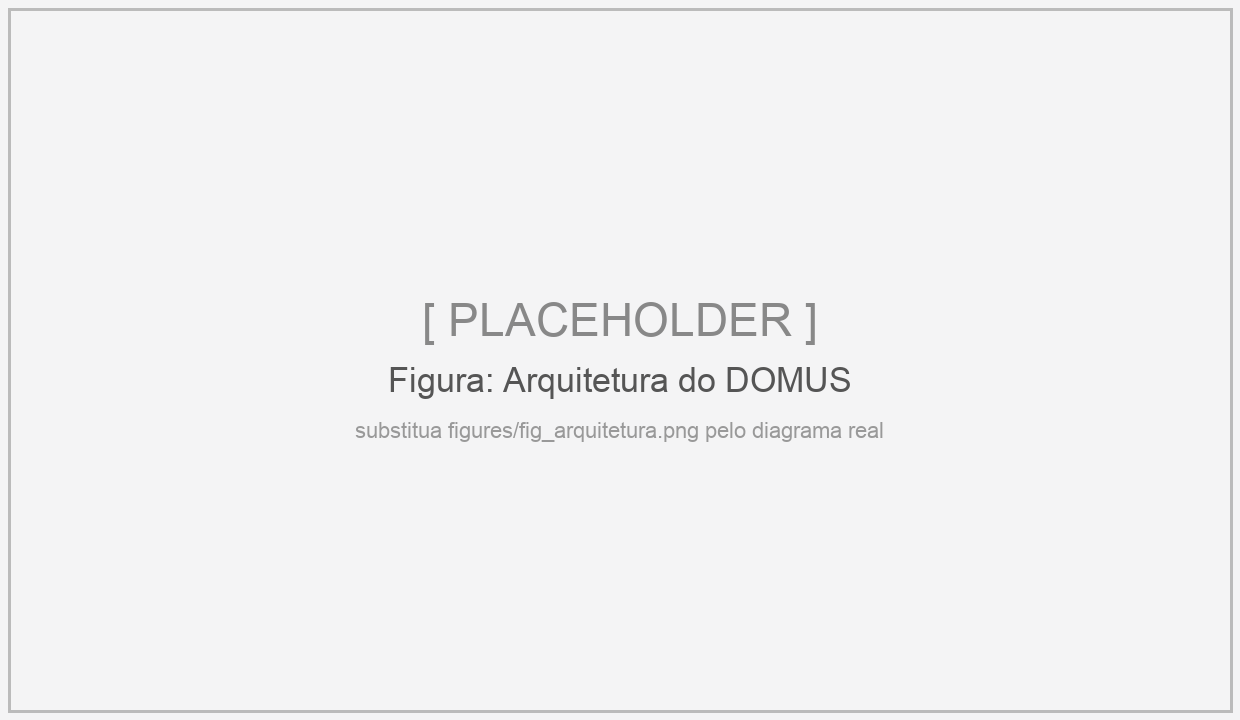
\includegraphics[width=0.9\textwidth]{fig_arquitetura}
\caption{Arquitetura em camadas do DOMUS: PWA, \emph{back end} modular e camada de \emph{adapters} sobre a rede local.}
\label{fig:arquitetura}
\end{figure}

\subsection{Padrão Adapter}

O princípio inegociável do projeto é que \emph{nenhum} \emph{controller} ou
serviço chama uma biblioteca de IoT diretamente: todo acesso ao \emph{hardware}
passa pela interface \texttt{DeviceAdapter}, definida em
\texttt{device-adapter.interface.ts}. O contrato expõe operações de ciclo de
vida (\texttt{connect}/\texttt{disconnect}), de atuação (\texttt{turnOn},
\texttt{turnOff}, \texttt{toggle}, \texttt{setBrightness}, \texttt{setColor},
\texttt{setColorTemp}) e de leitura (\texttt{readState}, \texttt{readEnergy}).
Capacidades não suportadas por um dispositivo lançam
\texttt{NotImplementedException}; e o código distingue explicitamente duas
falhas: \texttt{DeviceOfflineError} (o dispositivo não respondeu) e
\texttt{DeviceCommandError} (respondeu, mas rejeitou o comando) --- distinção
que evita marcar como ``\emph{offline}'' um aparelho que apenas recusou uma
credencial.

Uma \emph{factory} (\texttt{DeviceAdapterFactory}) escolhe a implementação
concreta pelo campo \texttt{protocol} do dispositivo e monta o
\texttt{AdapterContext}, descriptografando os segredos apenas nesse instante e
em memória. As implementações concretas são:

\begin{itemize}
  \item \textbf{TuyaAdapter} --- usa a biblioteca \texttt{tuyapi} sobre TCP na
    porta 6668. Mantém uma conexão persistente (o dispositivo aceita apenas uma
    conexão local por vez) e mapeia as capacidades para os \emph{data points}
    (DPS) do protocolo, com conversões de escala e de espaço de cor
    (Tabela~\ref{tab:dps}). Toda chamada de rede é limitada a 5~s (TUYA, 2025).
  \item \textbf{TapoAdapter} --- usa \texttt{tp-link-tapo-connect} com
    \emph{re-login} automático em caso de sessão expirada. Converte as unidades
    cruas de energia da tomada P110 (potência em mW; energia em Wh) para W e
    kWh, e retorna \texttt{null} em leitura não confiável para não distorcer as
    médias do painel (TP-LINK, 2024).
  \item \textbf{MockAdapter} --- simula um dispositivo em memória. É de uso
    obrigatório: o sistema inteiro roda e é testado sem \emph{hardware}, o que
    desacopla o desenvolvimento da disponibilidade física dos aparelhos.
\end{itemize}

Além desses, o repositório declara dois \emph{adapters} aditivos ---
\texttt{TuyaCloudAdapter} (Tuya Open API) e \texttt{HomeAssistantAdapter} (REST
de uma instância existente) --- que validam a extensibilidade do padrão sem
alterar o núcleo. A Tabela~\ref{tab:adapters} sintetiza os protocolos e sua
situação de maturidade.

\begin{table}[H]
\centering
\caption{Protocolos suportados pela camada de \emph{adapters}.}
\label{tab:adapters}
\begin{tabular}{@{}llll@{}}
\toprule
\textbf{Protocolo} & \textbf{Biblioteca} & \textbf{Transporte} & \textbf{Situação} \\
\midrule
\textsc{Tapo}  & \texttt{tp-link-tapo-connect} & LAN (KLAP)      & Controle local pleno \\
\textsc{Tuya}  & \texttt{tuyapi}               & LAN (TCP 6668)  & Comissionamento em validação \\
\textsc{Mock}  & ---                           & memória         & Pleno (testes e \emph{demo}) \\
Tuya Cloud     & Tuya Open API                 & nuvem           & Aditivo (valida sem \emph{hardware}) \\
Home Assistant & REST API + \emph{token}       & instância HA    & Aditivo (integração) \\
\bottomrule
\end{tabular}
\end{table}

\begin{table}[H]
\centering
\caption{Mapeamento de capacidades para \emph{data points} (DPS) Tuya no \texttt{TuyaAdapter}.}
\label{tab:dps}
\begin{tabular}{@{}llll@{}}
\toprule
\textbf{Capacidade} & \textbf{DPS} & \textbf{Faixa Tuya} & \textbf{Faixa DOMUS} \\
\midrule
Liga/desliga      & 20 & booleano        & \texttt{on}/\texttt{off} \\
Brilho            & 22 & 10--1000        & 0--100 (\%) \\
Temperatura de cor& 23 & 0--1000         & 2700--6500~K \\
Cor               & 24 & HSV \emph{hex}  & \texttt{\#RRGGBB} \\
\bottomrule
\end{tabular}
\end{table}

\subsection{Pipeline de voz}

O controle por voz segue uma cadeia de responsabilidades bem delimitada. O PWA
captura o áudio no celular (WebM/Opus, limitado a 5~MB, \textasciitilde3~s) e o
envia por \texttt{POST /voice/command} --- podendo alternativamente enviar texto
puro. No \emph{hub}, o áudio é transcrito por Whisper rodando localmente
(RADFORD et al., 2022): a implementação \texttt{WhisperSttService} usa
\texttt{nodejs-whisper} (\emph{bindings} de \texttt{whisper.cpp} em CPU), grava um
arquivo temporário apenas para a transcrição e o apaga em seguida, sem jamais
persistir o áudio (BRASIL, 2018). A transcrição alimenta o
\texttt{VoiceCommandParser}, que normaliza o texto (\emph{lowercase}, remoção de
acentos), detecta a intenção (ligar, desligar, alternar, ajustar brilho ou cor)
e casa o dispositivo por similaridade tolerante a erros de reconhecimento ---
usando distância de edição Damerau-Levenshtein e um esquema de pesos em que o
\emph{nome/apelido} do aparelho pesa mais que o cômodo e a palavra de tipo
(``tomada'', ``luz'') funciona como \emph{slot} que prioriza aparelhos daquele
tipo, à maneira de assistentes comerciais.

Se a confiança supera o limiar (0{,}6), o \texttt{VoiceService} chama
\texttt{executeCommand}, que entra na fila serializada por dispositivo
(\texttt{DeviceCommandQueue}): comandos ao mesmo \texttt{deviceId} são
processados em série (a lâmpada Tuya aceita uma conexão por vez), enquanto
dispositivos distintos correm em paralelo. Cada comando de voz é registrado na
tabela \texttt{voice\_commands} com transcrição, intenção, confiança, sucesso e
latência (\texttt{latencyMs}), o que fornece a base empírica das métricas do
trabalho. No PWA, sinais sonoros curtos (\emph{earcons}) indicam os estados
``ouvindo'', ``processando'', ``executado'' e ``erro'', dando \emph{feedback}
imediato enquanto a rede responde (DETERDING et al., 2011).
% VERIFICAR: apontar o componente do PWA que dispara os earcons (apps/web/...).

A avaliação sobre 138 comandos reais mostrou acurácia de intenção de
\textbf{87{,}7\%} e latência mediana (p50) de \textbf{463~ms} (p95 de 2140~ms),
com um \emph{outlier} de 12{,}3~s correspondente ao \emph{timeout} de um
dispositivo \emph{offline}. A taxa de \emph{execução} bem-sucedida foi de
66{,}7\%, dominada não por erros do \emph{parser}, mas pela indisponibilidade de
\emph{hardware} (ver \S~\ref{cap:desenvolvimento}). O Whisper apresentou
alucinações típicas em trechos sem fala clara, como a transcrição espúria
``\texttt{[Som de futebol]}''.
% A análise completa (por que 87,7% de intenção mas 66,7% de execução) fica no
% capítulo de Resultados; aqui é evidência de que o pipeline funciona fim a fim.

\subsection{Comissionamento e controle local}

A entrada de um dispositivo começa pela descoberta na LAN
(\texttt{NetworkScannerService}), que combina três sinais de forma passiva e
sem depender de nuvem: (i) escuta do \emph{broadcast} UDP que aparelhos Tuya
emitem nas portas 6666/6667 (decifrado com a chave fixa do protocolo, revelando
o \emph{device id} e a versão); (ii) varredura TCP da sub-rede nas portas
típicas de IoT (80, 443, 6668, 9999); e (iii) identificação do fabricante pelo
prefixo OUI do endereço MAC lido da tabela ARP. O resultado é uma lista de
candidatos com palpite de protocolo, já pronta para o cadastro.

A diferença crucial entre os dois protocolos-alvo está no comissionamento. O
\textbf{Tapo} é controlável em sua \emph{forma plena}: bastam as credenciais de
consumidor (e-mail e senha da conta TP-Link) para o \texttt{loginDeviceByIp}
autenticar no protocolo KLAP diretamente na LAN, sem etapa intermediária. Já o
\textbf{Tuya} exige a \texttt{local\_key} e o \emph{Device ID} do aparelho ---
credenciais que o fabricante não expõe ao usuário final e que, na prática, só se
obtêm por caminhos indiretos. Esse é o \emph{gap} central do trabalho: o
comissionamento da lâmpada Intelbras EWS~410 permaneceu \textbf{bloqueado},
constituindo evidência empírica da barreira que ecossistemas proprietários
impõem ao controle local. A integração Tuya está, portanto, marcada como
\emph{em validação}, enquanto o controle local do Tapo foi comprovado com
latências medidas de \textbf{201--332~ms} por comando.

% [...] — Detalhar aqui, se o aluno reproduzir, o caminho tentado para extrair a
% local_key (app SmartLife/pareamento, harness de bootstrap) e por que falhou.

\subsection{Segurança e privacidade}

O DOMUS foi construído sob a premissa de que dados sensíveis nunca trafegam ou
repousam em texto puro. O acesso à API é protegido por JWT, e todo dado de
usuário é isolado por escopo: cada consulta filtra por \texttt{userId} e as
relações usam \texttt{onDelete: Cascade}, de modo que um usuário jamais alcança
dados de outro. Os segredos de dispositivo --- a \texttt{local\_key} Tuya e a
senha Tapo --- são cifrados com \textbf{AES-256-GCM} antes de persistir, no
formato \texttt{ivHex:authTagHex:cipherHex} (IV de 12 bytes, chave de 32 bytes
vinda do ambiente). Esses segredos nunca são registrados em \emph{log}: o
próprio \texttt{CryptoService} evita imprimir o \emph{payload} cifrado, e a
descriptografia ocorre somente na \emph{factory}, em memória, no momento do uso.
Quanto à voz, o áudio é tratado como efêmero --- gravado apenas para a
transcrição e apagado logo depois ---, em conformidade com a LGPD
(BRASIL, 2018).

\subsection{Cenas e rotinas}

Cenas e rotinas compartilham o mesmo executor de ações, o \texttt{ActionsRunner}.
Uma \textbf{cena} (\texttt{Scene}) é uma lista ordenada de ações persistida em
JSON; ao ser ativada, o \texttt{ScenesService} percorre as ações em ordem,
respeitando o \texttt{delaySeconds} de cada passo, e delega cada uma ao
\texttt{DevicesService} --- portanto, à fila serializada por dispositivo. Uma
ação que falha não interrompe as demais: o erro é registrado e a execução
prossegue, devolvendo ao final o resultado de cada passo.

As \textbf{rotinas} (\texttt{Automation}) acrescentam agendamento. O
\texttt{AutomationsService} converte a configuração de horário em uma expressão
\emph{cron} e registra um \texttt{CronJob} no \emph{scheduler} do NestJS; ao
subir, o \emph{hub} reagenda todas as automações habilitadas. Antes de persistir,
a expressão é validada, evitando gravar uma rotina inagendável; e, no disparo, as
\emph{condições} (faixa de horário, dia da semana) são avaliadas antes de
executar as ações. Cada disparo emite um evento por WebSocket, que o PWA usa para
refletir a mudança de estado sem \emph{polling}.

\subsection{PWA offline}

A escolha por um PWA (ADR-002) --- em vez de aplicativo nativo --- reforça a tese
\textit{local-first}: o aplicativo é instalado no celular (``adicionar à tela
inicial''), fala com o \emph{hub} pela rede local e não depende de servidores na
nuvem para funcionar no dia a dia. O estado do servidor é gerenciado com TanStack
Query, que mantém em \emph{cache} a última leitura conhecida dos dispositivos,
permitindo que a interface continue exibindo o painel mesmo em oscilações de
conectividade, enquanto os eventos por WebSocket ressincronizam o estado assim
que a conexão volta.
% [...] — Confirmar e descrever a estratégia de service worker / manifest do PWA
% (apps/web): o que é pré-cacheado (\emph{app shell}), política de \emph{cache} das
% chamadas à API e comportamento quando o hub está inacessível. Incluir aqui, se
% houver, captura de tela do app instalado.

Em síntese, o desenvolvimento entregou um núcleo funcional e testável sem
\emph{hardware}, com controle local comprovado para o Tapo e um caminho de voz
completo em português; as lacunas remanescentes --- notadamente o
comissionamento Tuya --- são discutidas como resultado no próximo capítulo,
juntamente com as métricas ainda a coletar (WER da transcrição, usabilidade por
SUS e custo total via BOM).

%========================================================
% CAPÍTULO 6 — RESULTADOS E DISCUSSÃO
% Incluído via \input em main.tex. NÃO adicionar preâmbulo.
% Separar sempre resultado CONFIRMADO (medido e sincronizado) de [a coletar].
%========================================================
\section{Resultados e discussão}\label{cap:resultados}

Este capítulo confronta os critérios de sucesso fixados na Seção~\ref{sec:protocolo}
com o que foi efetivamente medido no protótipo DOMUS. Adota-se, por rigor, uma
distinção explícita entre \textit{resultados confirmados} --- obtidos por medição
instrumentada e verificados em hardware ou no banco de dados do \textit{hub} --- e
métricas \textit{em coleta}, cujo procedimento está definido, porém cuja aquisição
ainda estava em andamento no fechamento desta versão. O Quadro~\ref{tab:panorama}
resume esse estado. A opção por declarar o que ainda não foi medido, em vez de
preencher lacunas com estimativas, é coerente com a postura de honestidade documental
assumida no trabalho e evita que a discussão confunda promessa de projeto com
evidência empírica. Vale registrar que as métricas de voz confirmadas não permanecem
apenas no banco: o próprio sistema as expõe em um painel de \textit{Resultados} que as
recalcula ao vivo a partir da tabela \texttt{voice\_commands} e distingue visualmente o
que é medido do que está em coleta --- transportando para dentro do produto a mesma
honestidade documental adotada aqui.

\begin{table}[H]
\centering
\caption{Panorama dos critérios de avaliação e seu estado de coleta.}
\label{tab:panorama}
\begin{tabular}{@{}lll@{}}
\toprule
\textbf{Critério} & \textbf{Instrumento} & \textbf{Estado} \\
\midrule
Controle local de hardware   & Latência KLAP (Tapo P110)        & Confirmado \\
Acurácia de intenção de voz  & \textit{Log} \texttt{voice\_commands} & Confirmado \\
Sucesso de execução de voz   & \textit{Log} \texttt{voice\_commands} & Confirmado \\
Latência voz$\rightarrow$ação & Percentis p50/p95                & Confirmado \\
Taxa de erro de palavra (WER) & Corpus controlado                & A coletar  \\
Custo total (BOM)            & Planilha datada, 2 cenários      & A coletar  \\
Usabilidade (SUS)            & Questionário, $n=3$--$5$         & A coletar  \\
Economia de energia          & Série antes/depois com carga     & A coletar  \\
Comissionamento sem \textit{app} & Tapo (pleno) / EWS 410 (bloqueado) & Confirmado \\
\bottomrule
\end{tabular}
\end{table}

\subsection{Controle local de hardware}\label{sec:res-controle}

O critério mais elementar da tese --- controlar hardware de prateleira sem trânsito
obrigatório pela nuvem do fabricante --- foi \textbf{confirmado} para a tomada
inteligente TP-Link Tapo~P110. O adaptador correspondente estabelece a sessão
diretamente na rede local pelo protocolo proprietário KLAP (\textit{Key Local
Authentication Protocol}), negociando o \textit{handshake} de autenticação a partir de
credenciais de consumidor, sem recorrer aos servidores da TP-Link em regime permanente
(TP-LINK, 2024). Trata-se da materialização operacional do princípio \textit{local-first}
descrito por Kleppmann et~al.\ (2019): o plano de controle reside na instalação local.

As latências fim-a-fim das operações de comando, medidas na rede local do laboratório,
situaram-se na faixa de \textbf{201 a 332~ms} (Tabela~\ref{tab:latencia-tapo}). Esse
intervalo é imperceptível como atraso de interação para o usuário e comparável ao de
comandos que trafegariam pela nuvem em condição de rede favorável, com a vantagem de
não depender da conectividade externa --- justamente o gargalo estrutural identificado
na justificativa do trabalho, dado que apenas 22\% dos domicílios brasileiros dispõem
de conectividade satisfatória (CETIC.br, 2024).

\begin{table}[H]
\centering
\caption{Latências de controle local do Tapo P110 pelo protocolo KLAP (rede local).}
\label{tab:latencia-tapo}
\begin{tabular}{@{}lcc@{}}
\toprule
\textbf{Estatística} & \textbf{Latência (ms)} & \textbf{Observação} \\
\midrule
Menor latência observada  & 201   & Comando após sessão estabelecida \\
Maior latência observada  & 332   & Inclui renegociação de \textit{handshake} \\
Mediana (p50)             & [...] & A confirmar no \textit{log} \\
Amostras ($n$)            & [...] & A confirmar no \textit{log} \\
\bottomrule
\end{tabular}
\end{table}
% NOTA: a faixa 201–332 ms está CONFIRMADA. Preencher p50, n e, se possível, quebra por
% operação (ligar / desligar / leitura de energia) a partir dos tempos registrados nos
% adaptadores. Se houver série suficiente, considerar figura fig_latencia_tapo.pdf.

\subsection{Reconhecimento de voz}\label{sec:res-voz}

O \textit{pipeline} de voz foi avaliado sobre \textbf{138 comandos reais} registrados na
tabela \texttt{voice\_commands} durante o uso do protótipo, o que caracteriza uma
coleta em uso, e não em laboratório controlado. A Tabela~\ref{tab:voz} consolida as
métricas confirmadas. É central, para a leitura correta dos números, separar quatro
grandezas que a literatura e o senso comum tendem a fundir: a acurácia de reconhecimento
da fala (WER), a acurácia de \textit{intenção}, o sucesso de \textit{execução} e a
latência.

A \textbf{acurácia de intenção} --- fração dos comandos em que o \textit{parser}
extraiu corretamente a ação pretendida e seu alvo --- foi de \textbf{87,7\%}. O
resultado indica que o interpretador de linguagem natural em pt-BR desempenha o seu
papel de forma robusta mesmo sobre transcrições ruidosas. Já o \textbf{sucesso de
execução} --- fração dos comandos que resultaram na mudança de estado física
pretendida --- foi de apenas \textbf{66,7\%}. A diferença de mais de vinte pontos
percentuais entre as duas métricas \emph{não} decorre de falha do \textit{parser}: ela
é \textbf{dominada por hardware indisponível} no momento do comando (dispositivo
\textit{offline}, tomada sem energia, alvo fora da rede). Em outras palavras, o sistema
compreendeu a intenção, mas não pôde efetivá-la porque o dispositivo-alvo não estava
acessível --- uma falha de disponibilidade de hardware, não de reconhecimento. Essa
decomposição é a resposta direta à objeção previsível da banca de que ``a execução
ficou abaixo de dois terços'': o número mede a confiabilidade do parque físico
disponível durante a coleta, não a qualidade do interpretador.

\begin{table}[H]
\centering
\caption{Métricas confirmadas do \textit{pipeline} de voz ($n=138$ comandos reais).}
\label{tab:voz}
\begin{tabular}{@{}lcl@{}}
\toprule
\textbf{Métrica} & \textbf{Valor} & \textbf{Observação} \\
\midrule
Comandos instrumentados ($n$) & 138      & Tabela \texttt{voice\_commands} \\
Acurácia de intenção          & 87,7\%   & Intenção + alvo corretos \\
Sucesso de execução           & 66,7\%   & Limitado por hardware \textit{offline} \\
Latência p50                  & 463~ms   & Voz $\rightarrow$ ação \\
Latência p95                  & 2.140~ms & Cauda superior \\
Latência máxima (\textit{outlier}) & 12,3~s & \textit{Timeout} de hardware \\
WER (taxa de erro de palavra) & [...]    & A coletar (corpus controlado) \\
\bottomrule
\end{tabular}
\end{table}

Quanto à \textbf{latência voz$\rightarrow$ação}, a mediana (p50) de \textbf{463~ms}
confirma uma resposta perceptualmente imediata no caso típico. O percentil~95 de
\textbf{2.140~ms} revela uma cauda superior mais lenta, apenas ligeiramente acima do
patamar informal de dois segundos e explicável pelo custo de transcrição do
\textit{Whisper} no \textit{hub} somado ao tempo de resposta do dispositivo. O
\textbf{\textit{outlier} máximo de 12,3~s} não representa lentidão do reconhecimento:
corresponde a um \textbf{\textit{timeout} de hardware}, em que o adaptador aguardou até
o limite a resposta de um dispositivo que não respondeu --- mais uma manifestação do
mesmo gargalo de disponibilidade física discutido acima. Reportar a latência por
percentis, e não por média, é deliberado: a média seria contaminada por esses eventos
de \textit{timeout} e mascararia o comportamento real percebido pela maioria dos
comandos.

Um achado qualitativo merece registro por seu valor probatório espontâneo. Em pelo
menos um enunciado, o \textit{Whisper} produziu a transcrição alucinada
\texttt{"[Som de futebol]"} para um segmento sem fala inteligível. Longe de ser um
constrangimento a ocultar, o episódio é \textbf{evidência empírica de uma limitação
conhecida} do reconhecimento de fala de vocabulário aberto em larga escala: modelos do
tipo \textit{Whisper} tendem a ``alucinar'' rótulos plausíveis em trechos de silêncio
ou ruído (RADFORD et~al., 2022). O fato de a alucinação ter emergido no uso real, e não
em um teste adversarial construído, reforça a fidelidade da coleta e alimenta
diretamente a discussão de limitações e de robustez da demonstração (Seção~\ref{sec:res-comissionamento}
e Capítulo~\ref{cap:consideracoes}).

A \textbf{taxa de erro de palavra (WER)} permanece \textbf{a coletar}. Diferentemente
das métricas acima, ela exige um corpus controlado --- protocolo previsto de, no mínimo,
50 enunciados com pelo menos três falantes distintos e transcrição de referência ---,
acompanhado de uma matriz de confusão de intenções. Sem esse corpus, seria incorreto
reportar WER a partir dos 138 comandos de uso, que não possuem \textit{ground truth}
textual.
% INSERIR (semana de métricas): WER global e por falante + matriz de confusão de
% intenções. Considerar figura fig_matriz_confusao.pdf.

\begin{figure}[H]
\centering
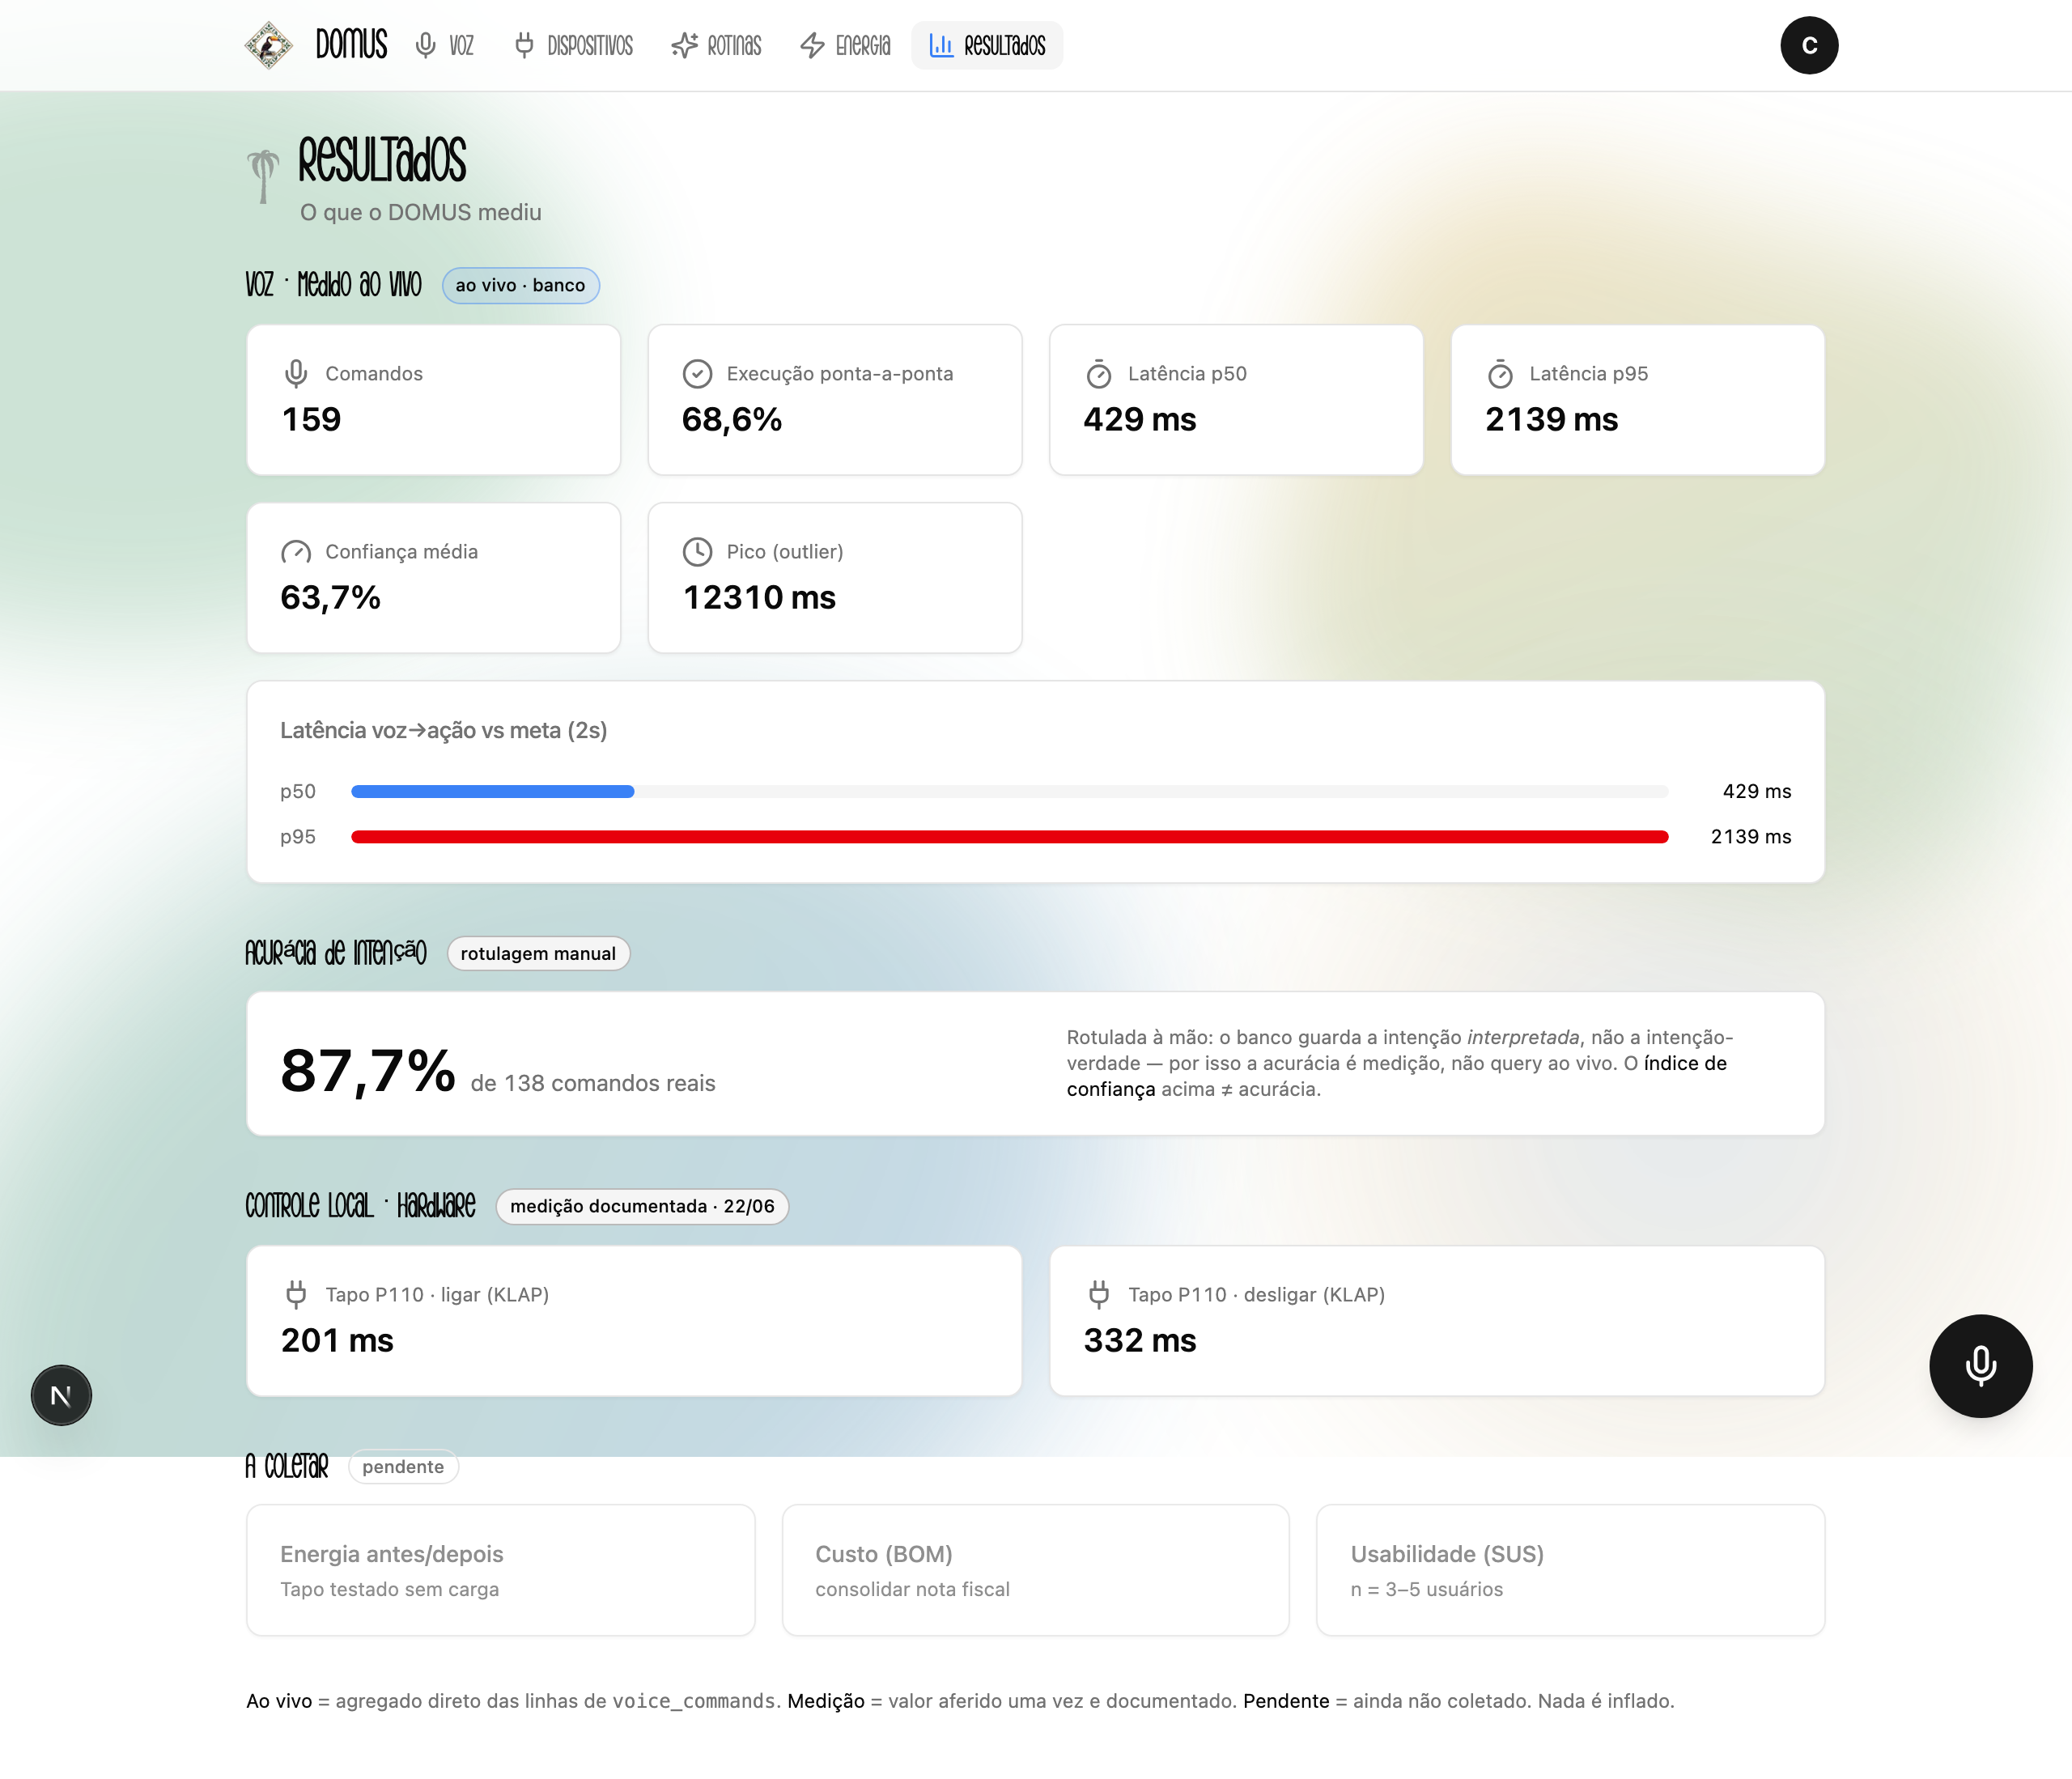
\includegraphics[width=0.82\textwidth]{05-resultados.png}
\caption{Painel de \textit{Resultados} do DOMUS: as métricas de voz são recalculadas ao
vivo a partir da tabela \texttt{voice\_commands}, distinguindo visualmente o que é
\emph{medido} do que está \emph{em coleta} --- a mesma honestidade documental desta seção.}
\label{fig:painel-resultados}
\end{figure}

\subsection{Custo (BOM)}\label{sec:res-custo}

O custo total de materiais (\textit{Bill of Materials}, BOM) é a métrica que sustenta
diretamente a alegação de ``baixo custo'' do título. Seu levantamento definitivo está
\textbf{a coletar}: exige uma planilha única e datada, com preços de varejo referenciados
(notas fiscais ou \textit{links}), estruturada em \textbf{dois cenários} que enfrentam
explicitamente a questão do \textit{hub} --- o item que a narrativa ingênua de custo
tende a esconder. A Tabela~\ref{tab:bom} apresenta o esqueleto a ser preenchido.

\begin{table}[H]
\centering
\caption{Custo de materiais (BOM) do DOMUS em dois cenários --- valores a coletar.}
\label{tab:bom}
\begin{tabular}{@{}lcc@{}}
\toprule
\textbf{Item} & \textbf{Incremental (R\$)} & \textbf{Completo (R\$)} \\
\midrule
TP-Link Tapo P110 (tomada)          & [...] & [...] \\
Intelbras EWS 410 (lâmpada)         & [...] & [...] \\
\textit{Hub} de processamento       & 0\,\textsuperscript{a} & [...]\,\textsuperscript{b} \\
Outros (cabos, fonte)               & [...] & [...] \\
\midrule
\textbf{Total}                      & \textbf{[...]} & \textbf{[...]} \\
\bottomrule
\end{tabular}

{\footnotesize\noindent\textsuperscript{a}~PC/notebook doméstico reaproveitado como
\textit{hub} (custo marginal zero). \quad
\textsuperscript{b}~Mini-PC ou Raspberry~Pi dedicado.\par}
\end{table}
% INSERIR os valores datados; discutir a meta informal de R$ 200 de custo INCREMENTAL,
% e o fato de que a divergência histórica (R$ 130 vs R$ 180 na documentação) se resolve
% justamente por explicitar se o hub entra ou não na conta.

A discussão central desta subseção, portanto, não é o preço da lâmpada ou da tomada
--- baratos e já premissa do trabalho ---, mas o \textbf{custo do \textit{hub}}. No
cenário \textit{incremental}, em que um computador doméstico ocioso é reaproveitado, o
custo marginal do \textit{hub} tende a zero e a meta de custo total incremental
inferior a R\$~200 é plausível. No cenário \textit{completo}, com um mini-PC ou
Raspberry~Pi dedicado, esse custo precisa ser contabilizado com honestidade, sob pena
de a alegação de democratização escamotear o seu principal item de despesa.

\subsection{Usabilidade (SUS)}\label{sec:res-sus}

A avaliação de usabilidade pela \textit{System Usability Scale} (SUS) está \textbf{a
coletar}. O protocolo previsto aplica o questionário SUS padrão a uma amostra de
$n = 3$ a $5$ participantes, após um roteiro de cinco tarefas representativas
(comissionar um dispositivo, emitir um comando de voz, criar uma automação por horário,
consultar o painel de energia e recuperar-se de uma falha simulada). A
Tabela~\ref{tab:sus} apresenta a estrutura de reporte.

\begin{table}[H]
\centering
\caption{Resultado da avaliação de usabilidade (SUS) --- a coletar.}
\label{tab:sus}
\begin{tabular}{@{}lc@{}}
\toprule
\textbf{Item} & \textbf{Valor} \\
\midrule
Participantes ($n$)          & [...] \\
Pontuação SUS média          & [...] \\
Desvio-padrão                & [...] \\
Faixa (mín.\ --- máx.)       & [...] \\
Interpretação qualitativa    & [...] \\
\bottomrule
\end{tabular}
\end{table}
% INSERIR: SUS por participante + média. Score >= 68 é a média de referência da escala;
% discutir com cautela dado o n pequeno. Reconhecer explicitamente que n=3–5 sustenta
% um argumento DIRECIONAL de usabilidade, não uma generalização — resposta preparada
% para a objeção de "democratização com n=1".

Reconhece-se, desde já, que uma amostra dessa magnitude não autoriza generalização
estatística. O propósito da medição é \textbf{direcional}: verificar se usuários sem
formação técnica conseguem completar as tarefas essenciais e identificar barreiras
grosseiras de usabilidade, alimentando a discussão de democratização em sua forma
prudente. Sem coleta de SUS, a defesa deve recuar para o título alternativo mais
conservador, centrado em viabilidade técnica.

\subsection{Energia}\label{sec:res-energia}

O painel de energia foi implementado e alimentado pela telemetria do Tapo~P110, que o
\texttt{EnergyService} coleta em intervalos regulares e persiste na tabela
\texttt{energy\_readings}, acumulando um volume expressivo de leituras. Sobre essa série,
o painel agrega o consumo \textbf{da casa inteira} --- somando todas as conexões que
medem energia --- e o apresenta em janelas de \textbf{24~h, 7 e 30~dias}, com resolução
que desce ao \textbf{minuto} na janela diária; complementa a leitura com a
\textbf{participação de cada conexão} no total e um \textbf{comparativo mês a mês}, além
do consumo por aparelho acessível ao abrir cada dispositivo.

\begin{figure}[H]
\centering
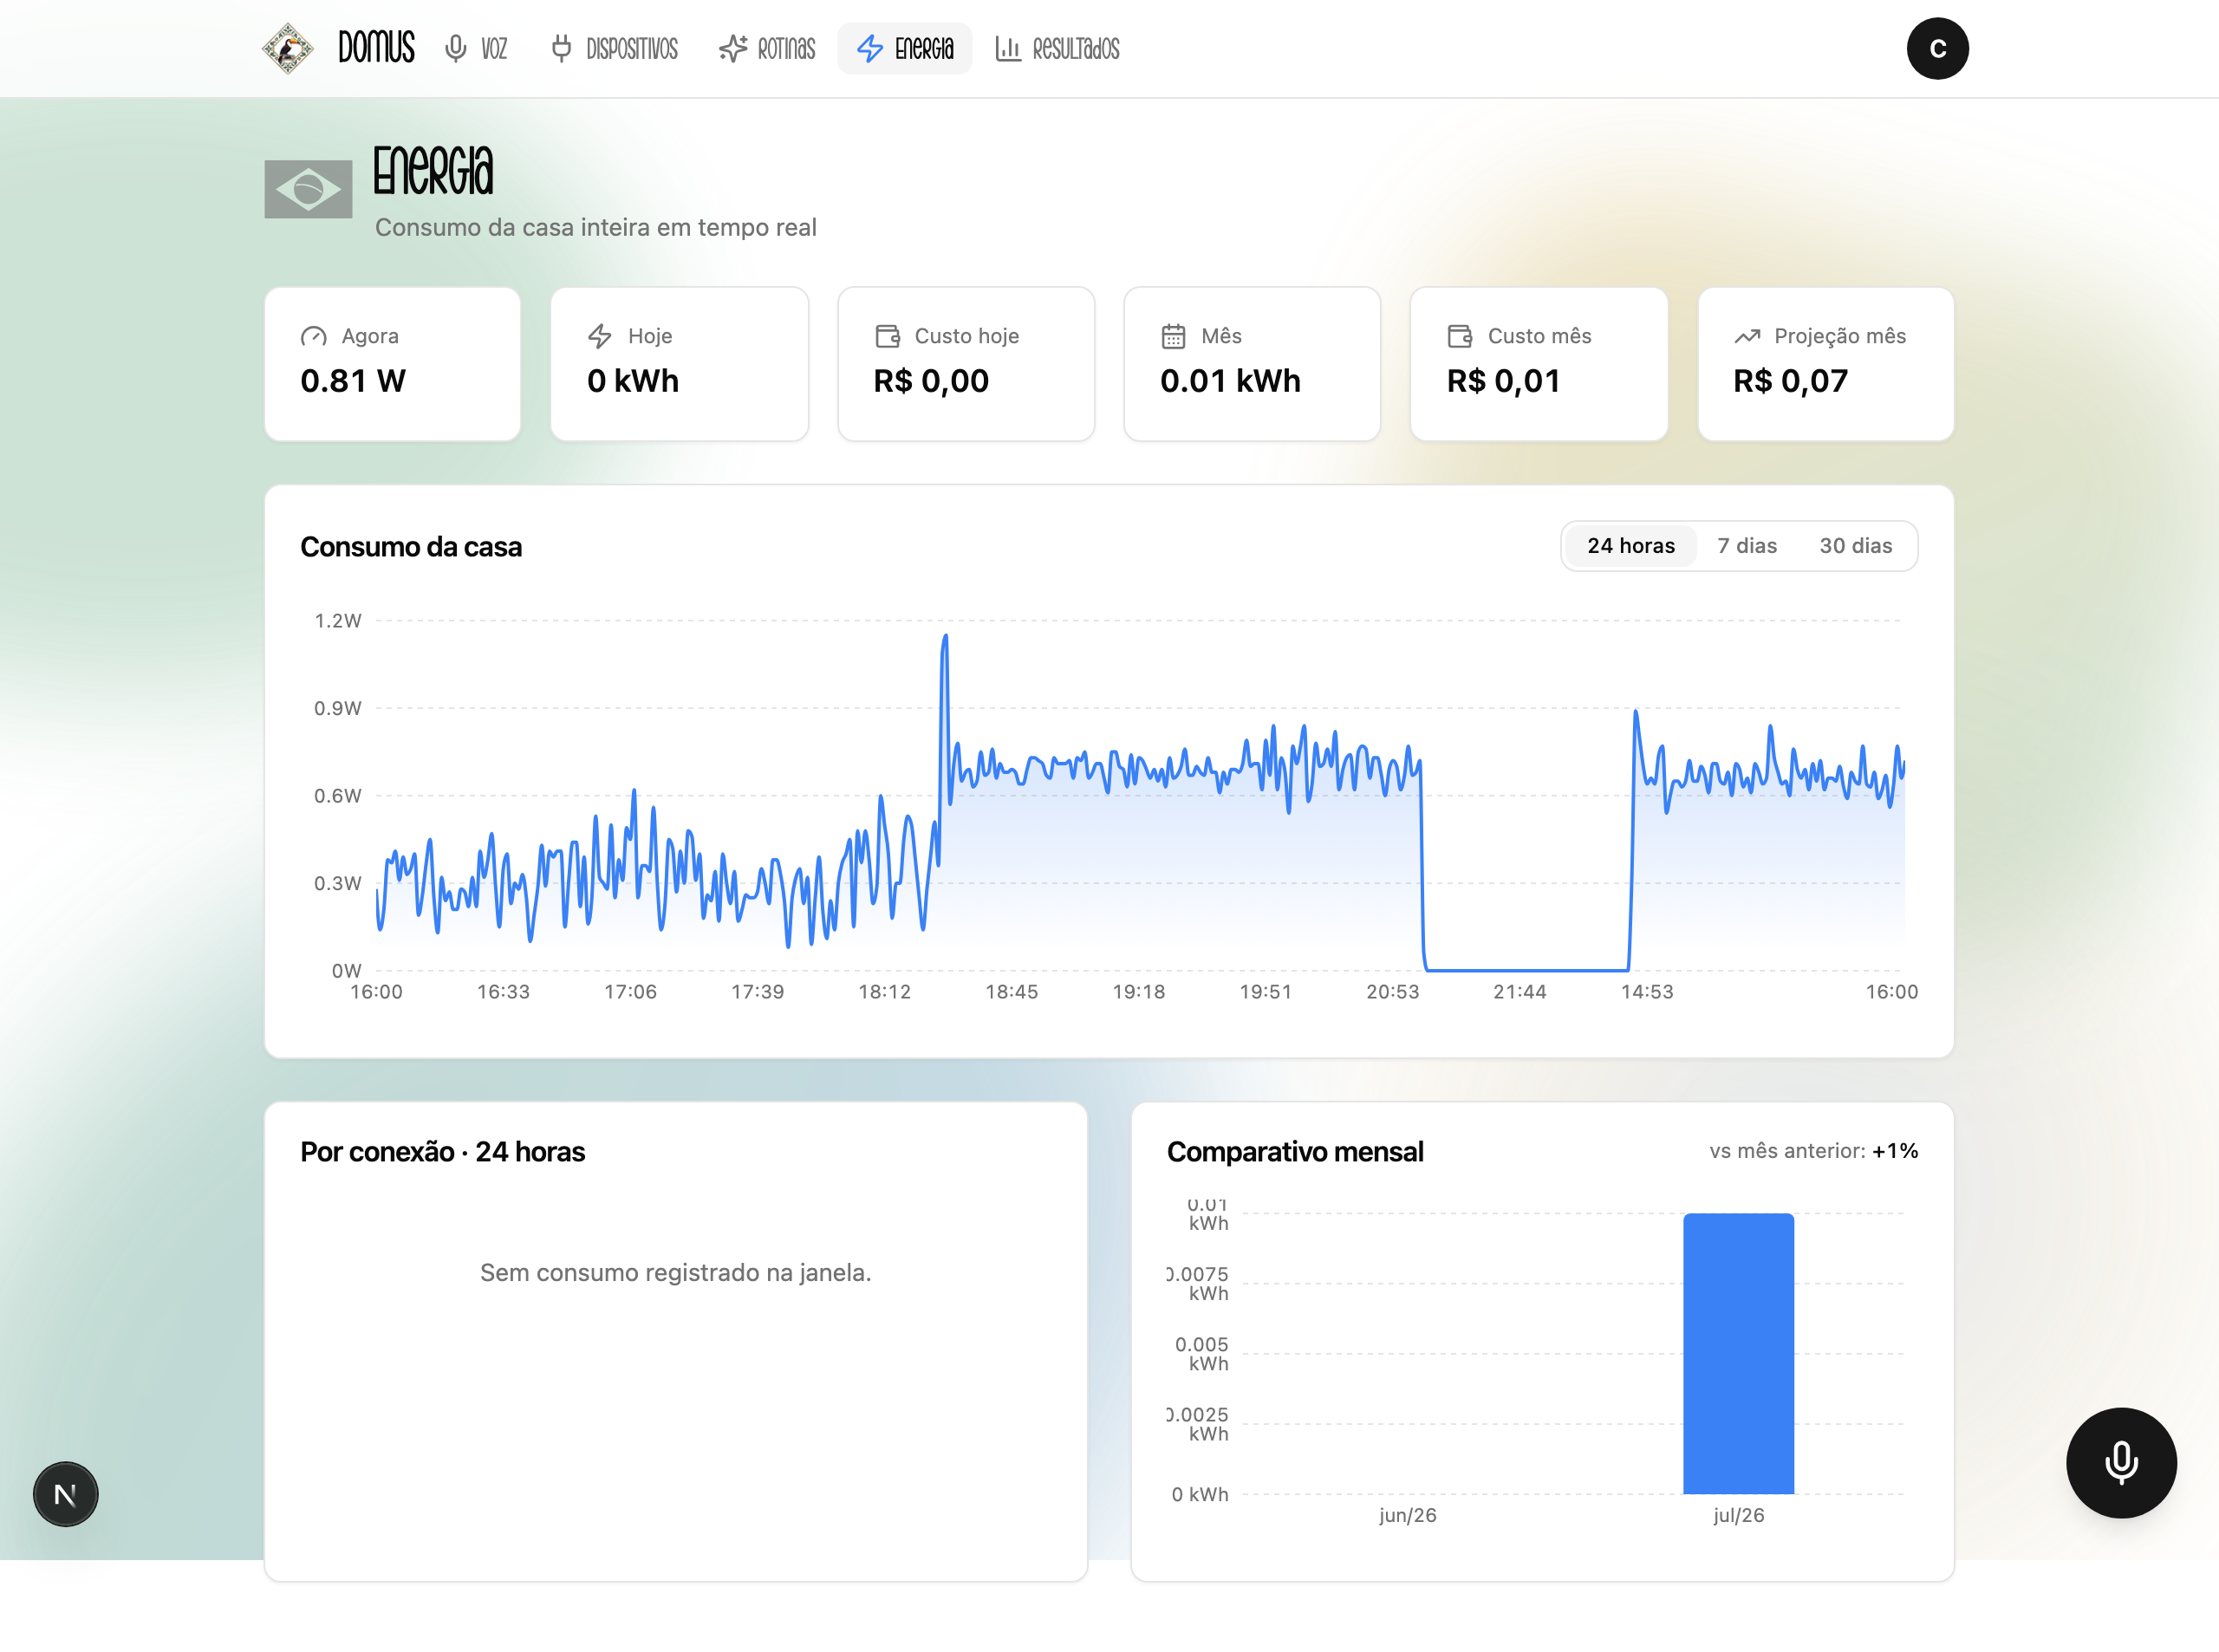
\includegraphics[width=0.82\textwidth]{04-energia.png}
\caption{Painel de energia da casa: consumo agregado com seletor de período (24~h em
resolução de minutos, 7 e 30 dias), participação por conexão e comparativo mensal,
alimentado pela telemetria real do Tapo~P110.}
\label{fig:painel-energia}
\end{figure}

Contudo, a avaliação de
\textbf{economia de energia} propriamente dita está \textbf{a coletar}, por uma razão
metodológica honesta: as leituras acumuladas foram obtidas com a tomada sem carga útil
acoplada (potência residual da ordem de fração de \textit{watt}), o que torna a série
inadequada para demonstrar economia real. A avaliação válida requer uma \textbf{série
temporal antes/depois com carga real} (por exemplo, um ventilador ou abajur submetido a
uma rotina de desligamento programado), coletada por um período mínimo de vários dias
consecutivos. A Tabela~\ref{tab:energia} apresenta a estrutura de reporte.

\begin{table}[H]
\centering
\caption{Consumo antes/depois da automação, com carga real --- a coletar.}
\label{tab:energia}
\begin{tabular}{@{}lccc@{}}
\toprule
\textbf{Condição} & \textbf{Período} & \textbf{Consumo (kWh)} & \textbf{Custo (R\$)} \\
\midrule
Antes (sem automação) & [...] & [...] & [...] \\
Depois (com automação) & [...] & [...] & [...] \\
\midrule
\textbf{Economia}     & --- & \textbf{[...]} & \textbf{[...]} \\
\bottomrule
\end{tabular}
\end{table}
% INSERIR: série >= 5–7 dias com carga real; tarifa em R$/kWh referenciada (não
% hardcoded). Se a série não for viável a tempo, REBAIXAR explicitamente para "painel
% demonstrado; economia não avaliada" nas limitações (§7.1), sem inflar o resultado.

Enquanto a série com carga não estiver disponível, o resultado honesto é: o
\emph{painel} de monitoramento de energia está \textbf{demonstrado e funcional}, porém a
\emph{economia} proporcionada pela automação \textbf{não foi avaliada}. Essa distinção
é mantida deliberadamente para não converter capacidade de medição em alegação de
benefício não comprovado.

\subsection{Validação com usuários}\label{sec:res-survey}

Para confrontar as premissas do trabalho --- sobretudo a de que a barreira dominante é o
\emph{comissionamento}, e não o preço --- com a percepção de usuários reais, aplicou-se um
questionário eletrônico (Apêndice~\ref{ap:survey}) a uma amostra de conveniência de
diferentes faixas etárias e regiões (Recife/PE, São Paulo, Rio de Janeiro e participantes
na Itália). Trata-se de uma avaliação \textbf{direcional} ($n = 8$--$15$), não de uma
inferência estatística. No fechamento desta versão, a coleta estava \textbf{em andamento}.
Os resultados consolidados serão reportados aqui em gráficos gerados a partir das respostas
reais: (i)~perfil etário e regional da amostra; (ii)~fração que já possui automação
\emph{versus} a que automatizaria se fosse simples e barata; e, sobretudo, (iii)~o
\emph{ranking das dificuldades percebidas}, cuja leitura será cruzada com o achado de
comissionamento (Seção~\ref{sec:res-comissionamento}) para testar, com evidência de
usuários, a hipótese central do trabalho.

% INSERIR (após a coleta no Google Forms): gerar dos dados REAIS e NÃO antes:
%  (a) barras horizontais do ranking de barreiras (Bloco 3 do instrumento);
%  (b) perfil etário/regional + % que já tem automação vs. automatizaria;
%  (c) SUS médio por faixa etária/cidade. Não reportar números sem coleta real.

\subsection{Comissionamento}\label{sec:res-comissionamento}

O comissionamento --- transformar hardware de prateleira em dispositivo controlável
sem recorrer ao aplicativo proprietário nem a portais de desenvolvedor --- é a
contribuição-título do trabalho, e os resultados aqui são \textbf{assimétricos e, por
isso mesmo, esclarecedores}.

No caminho \textbf{TP-Link Tapo}, a forma plena foi \textbf{demonstrada}: partindo de
credenciais de consumidor, o DOMUS estabelece controle local pelo protocolo KLAP
(Seção~\ref{sec:res-controle}), sem que o uso cotidiano dependa do \textit{app} do
fabricante ou de servidores externos (TP-LINK, 2024). Esse é o caso que sustenta a
forma \textit{forte} da tese em um dispositivo real.

No caminho \textbf{Intelbras/Tuya EWS 410}, o comissionamento foi \textbf{bloqueado no
provisionamento}. A lâmpada nunca chegou a ser controlada em hardware porque o fluxo
exigiu, na prática, credenciais de baixo nível (\textit{Device~ID} e
\textit{local\_key}) obtidas por meio do portal de desenvolvedor Tuya~IoT, cujo
emparelhamento de dispositivos esbarrou no \textbf{limite de dois \textit{slots} de
dispositivo} da plataforma em regime de avaliação (TUYA, 2025). Um \textit{harness} de
provisionamento local foi preparado, mas o gargalo permaneceu no ato de vincular o
dispositivo à conta da plataforma.

A leitura deste bloqueio é o ponto mais importante do capítulo. Ele \textbf{não é um
fracasso de engenharia a ser minimizado}: é a \textbf{evidência empírica mais forte da
própria tese}. A barreira de comissionamento que a Introdução postula como o real
obstáculo à democratização --- aplicativos proprietários, contas em nuvem, portais de
desenvolvedor em inglês e limites administrativos de plataforma --- foi \textbf{real a
ponto de bloquear até o autor do trabalho}, um desenvolvedor com acesso ao \textit{harness},
à documentação e ao ferramental. Se essa barreira detém quem a estuda, seu efeito sobre
o domicílio típico é qualitativamente mais severo, o que é consistente com a baixa
penetração de automação residencial no país (IBGE, 2024). O contraste entre o caminho
Tapo (pleno) e o caminho Tuya (bloqueado) converte-se, assim, de limitação em resultado:
demonstra simultaneamente que o objetivo é \textit{alcançável} (Tapo) e que a barreira
que ele ataca é \textit{concreta e mensurável} (Tuya). A validação plena do caminho Tuya
permanece em andamento e é retomada como limitação declarada no
Capítulo~\ref{cap:consideracoes}.
% NOTA: a promessa "sem app / sem portal" está DEMONSTRADA para Tapo e CARACTERIZADA
% como gap para Tuya. Não afirmar controle da EWS 410 em hardware. Se o timebox da EWS
% 410 for bem-sucedido antes da defesa, atualizar esta subseção para a forma forte.

%======================= CONSIDERAÇÕES FINAIS =======================
% Capítulo 7. Retoma a pergunta norteadora e a hipótese (§1.2), sintetiza o que o
% artefato demonstrou (Cap. 6) e delimita, com honestidade, o que permanece como
% hipótese. Estrutura: retomada da hipótese (forma fraca x forte) -> limitações ->
% trabalhos futuros. Cite apenas o conjunto canônico de referências.
\section{Considerações finais}\label{cap:consideracoes}

Este trabalho partiu de uma constatação incômoda: no Brasil, o hardware de automação
residencial já é barato --- uma lâmpada ou tomada Wi-Fi genérica do ecossistema Tuya
custa entre R\$~30 e R\$~60 ---, mas transformar esse hardware em automação utilizável
permanece inacessível ao domicílio típico. A penetração de dispositivos inteligentes
subiu apenas de 14,3\% (2022) para 16,4\% (2024) dos domicílios, contra cerca de 44\%
nos Estados Unidos e no Reino Unido, e com forte corte regional e de renda (IBGE, 2024).
A tese central defendida foi que essa exclusão decorre menos do \emph{preço de compra}
e mais da \emph{barreira de comissionamento} --- a exigência de aplicativos
proprietários, contas em nuvem e portais de desenvolvedor em inglês para colocar o
aparelho em operação ---, agravada por uma dependência estrutural de conectividade que
só 22\% dos domicílios possuem de forma satisfatória (CETIC.br, 2024). O princípio
operacional adotado como resposta foi ``nuvem uma vez, local para sempre''.

A partir dessa tese, o DOMUS foi concebido como uma prova de conceito de \textit{hub}
de automação \textit{local-first}, controlável por voz em português brasileiro
processada no próprio \textit{hub}, e construído sobre o padrão \textit{Adapter} para
isolar a heterogeneidade de protocolos. As seções seguintes retomam a hipótese de
pesquisa formulada na Seção~\ref{cap:intro}, respondem-na separando o que foi
efetivamente demonstrado do que permanece como conjectura, e delimitam as limitações e
os desdobramentos do estudo.

\subsection{Retomada da hipótese: forma fraca e forma forte}

A hipótese central --- \emph{a democratização da automação residencial depende da
redução da barreira de comissionamento, e não do custo do hardware} --- foi, no
Capítulo~\ref{cap:resultados}, reformulada como uma alegação de viabilidade
falsificável, verificável dispositivo a dispositivo: \emph{é tecnicamente viável
comissionar e controlar localmente, sem aplicativo do fabricante e sem portais de
desenvolvedor, dispositivos Wi-Fi genéricos de baixo custo, com comandos de voz em
português processados integralmente no \textit{hub}, a custo incremental inferior a
R\$~200}. Para responder a essa hipótese com honestidade, é preciso distingui-la em
duas formas de força argumentativa distinta.

\subsubsection{Forma fraca --- demonstrada}

Na sua forma fraca --- \emph{a viabilidade técnica do controle local por voz em
português brasileiro, sem dependência permanente de nuvem} ---, a hipótese está
\textbf{demonstrada}. O resultado mais sólido é o controle local da tomada TP-Link
Tapo~P110 pelo protocolo KLAP, com operações de liga/desliga bem-sucedidas a latências
de 201--332~ms; como cada operação é confirmada por leitura de estado e a
indisponibilidade produz erro explícito, o sucesso comprova comunicação real com o
aparelho, afastando a hipótese de simulação silenciosa. Esse caminho é a demonstração
plena da tese: as credenciais utilizadas são de \emph{consumidor} (as mesmas do
aplicativo comum), não de desenvolvedor, e ainda assim habilitam controle inteiramente
local (TP-LINK, 2024). O reconhecimento de fala, por sua vez, roda no próprio
\textit{hub} via \textit{Whisper} (RADFORD et al., 2022), descartando o áudio após a
transcrição, em coerência com o princípio de minimização (BRASIL, 2018): sobre 138
comandos de voz reais instrumentados, a acurácia de \emph{intenção} foi de 87,7\%, com
latência ponta-a-ponta de 463~ms na mediana (p50) e 2.140~ms no percentil~95 (p95). A
arquitetura, portanto, sustenta o que se propôs a sustentar: um plano de controle ---
\textit{Whisper}, adaptadores, chaves e dados --- que existe apenas na instalação local,
com a nuvem confinada ao papel de vitrine, na acepção de \textit{local-first} de
Kleppmann et al. (2019).

\subsubsection{Forma forte --- ainda hipótese}

Na sua forma forte --- \emph{a democratização efetivamente realizada}, isto é, a
automação tornada acessível ao usuário não técnico e de baixa renda ---, a hipótese
\textbf{permanece como conjectura}, e o trabalho é deliberadamente honesto quanto a
isso. Três lacunas sustentam essa ressalva. Primeiro, a própria contribuição que dá
nome ao trabalho --- comissionar sem aplicativo do fabricante e sem portal de
desenvolvedor --- só foi demonstrada plenamente no caminho Tapo; a lâmpada Intelbras/Tuya
EWS~410 nunca foi controlada em hardware, e seu comissionamento local permaneceu
\emph{bloqueado} ao longo do estudo. Longe de ser mero fracasso, esse bloqueio constitui
\textbf{evidência empírica da própria barreira que a tese nomeia}: se o comissionamento
de um dispositivo Wi-Fi genérico é complexo a ponto de resistir ao autor do sistema
--- que dispõe de documentação, ferramentas e do harness pronto ---, então ele é, com
folga, complexo demais para o domicílio-alvo. Segundo, três dos quatro critérios de
sucesso definidos na metodologia --- taxa de erro de palavra (WER) sobre corpus
rotulado, escala de usabilidade (SUS) com o público-alvo e o custo total consolidado em
uma lista de materiais (BOM) --- ainda não foram coletados, de modo que as afirmações de
\emph{acessibilidade} e de \emph{economia} não estão autorizadas pelos dados. Terceiro,
mesmo a métrica de voz precisa ser lida com cautela: a taxa de sucesso de
\emph{execução} foi de apenas 66,7\%, mas essa queda é dominada por \emph{hardware
offline}, não pelo interpretador de comandos --- o \textit{outlier} de latência máxima,
de 12,3~s, corresponde a um \textit{timeout} de hardware, não a lentidão do
processamento de linguagem. Registrou-se, ainda, ao menos uma alucinação do
\textit{Whisper}, que transcreveu ruído de fundo como ``[Som de futebol]'', ilustrando a
tensão real entre custo e acurácia num modelo pequeno rodando em \textit{hardware}
modesto.

A Tabela~\ref{tab:sintese-hipotese} sintetiza essa partição entre o demonstrado e o
pendente.

\begin{table}[H]
\centering
\caption{Síntese da resposta à hipótese: o que foi demonstrado e o que permanece
conjectura ao encerramento do estudo.}
\label{tab:sintese-hipotese}
\small
\begin{tabular}{@{}p{3.8cm}p{2.3cm}p{8.2cm}@{}}
\toprule
\textbf{Alegação} & \textbf{Estado} & \textbf{Evidência / pendência} \\
\midrule
Controle local sem nuvem (Tapo P110) & Demonstrada & Latências 201--332~ms via KLAP;
confirmação por leitura \\
Voz pt-BR processada no \textit{hub} & Demonstrada & Intenção 87,7\% em 138 comandos;
áudio descartado \\
Latência de voz aceitável & Parcial & p50 463~ms / p95 2.140~ms; \textit{outlier} 12,3~s
= \textit{timeout} de hardware \\
Comissionamento Tuya sem app/portal & Em validação & EWS~410 bloqueada --- evidência
empírica da barreira \\
Acurácia de fala (WER) & A coletar & [WER] --- corpus rotulado pendente \\
Acessibilidade ao público-alvo & A coletar & [SUS] --- teste com $n=3$--5 pendente \\
Custo incremental $<$ R\$~200 & A coletar & [BOM] datada, 2 cenários (com/sem \textit{hub}) \\
\bottomrule
\end{tabular}
\end{table}
% Preencher [WER], [SUS] e [BOM] após a semana de coleta de métricas.

Em suma, o estudo responde afirmativamente à \emph{pergunta norteadora} na dimensão
técnica e mantém como hipótese aberta a dimensão socioeconômica: demonstra-se que a
arquitetura proposta \emph{pode} sustentar automação local, barata e por voz, mas ainda
não se demonstra que ela \emph{de fato} democratiza o acesso --- daí o caráter
\emph{direcional} do título, que aponta para um objetivo perseguido, não para um
resultado já alcançado.

\subsection{Limitações}\label{sec:limitacoes}

O trabalho está sujeito às seguintes limitações, declaradas de forma explícita para
delimitar o alcance das conclusões:

\begin{enumerate}
  \item \textbf{Comissionamento da lâmpada Wi-Fi não concluído em hardware.} O
  provisionamento da Intelbras/Tuya EWS~410 permaneceu bloqueado; o controle da lâmpada
  física --- incluindo brilho e cor --- não foi exercido em hardware ao longo do estudo,
  e a validação do adaptador Tuya deu-se contra um dispositivo que expõe o mesmo modelo
  de dados, não contra o aparelho físico-alvo (TUYA, 2025).

  \item \textbf{Consumo de energia sem série com carga real.} O painel de energia
  agrega leituras da Tapo~P110, porém a tomada foi operada sem carga significativa
  durante a coleta; as afirmações de ``economia antes/depois'' não estão sustentadas por
  série temporal com um aparelho consumindo potência apreciável, e a tarifa de energia
  utilizada é um valor fixo de referência. O painel deve, portanto, ser lido como
  \emph{demonstrado}, e a economia como \emph{não avaliada}.

  \item \textbf{Funcionalidades de organização sem endpoint.} Os conceitos de cômodos
  (\textit{Rooms}) e de multiusuário (\textit{Users}) existem no modelo de dados, mas
  não dispõem de controladores/endpoints completos; permanecem como estrutura preparada,
  não como funcionalidade exercitável de ponta a ponta.

  \item \textbf{Adaptadores físicos fora da cobertura de testes, por \emph{design}.} A
  cobertura automatizada (aproximadamente [...\%]) % inserir a cobertura real reportada no Cap. 6 (ex.: 88,1%)
  apoia-se no adaptador MOCK; os adaptadores que falam com \textit{hardware} real não
  possuem testes unitários dedicados, por decisão de projeto que veda testes dependentes
  de hardware físico no ambiente de integração contínua. A validação desses adaptadores
  é empírica, não automatizada.

  \item \textbf{Retenção de transcrições suspensa e consentida durante o estudo.} A
  política de retenção mínima descrita no projeto --- descarte imediato da transcrição
  após a execução e expurgo diário do log de auditoria --- \emph{não} esteve ativa
  durante a fase de coleta: as 138 transcrições foram deliberadamente mantidas, mediante
  consentimento informado, para viabilizar as métricas do Capítulo~\ref{cap:resultados}.
  Trata-se de retenção configurável, habilitada de forma temporária e justificada à luz
  da base legal do consentimento (BRASIL, 2018); a purga automática permanece como
  intenção de projeto, não como comportamento implementado.

  \item \textbf{``Local-first'' por configuração, não por contingência automática.} No
  DOMUS, o controle local é o caminho \emph{primário por configuração}, e a falha do
  controle local produz \emph{aviso ao usuário} --- não uma queda silenciosa para a
  nuvem. Não há, portanto, \textit{fallback} automático local~$\rightarrow$~nuvem no
  sentido pleno da literatura de \textit{local-first} (KLEPPMANN et al., 2019); a
  garantia oferecida é a de que, se o controle local quebrar, o sistema avisa, e não a
  de reconvergência automática de estado entre réplicas.

  \item \textbf{Título direcional.} Conforme discutido acima, o título afirma uma
  contribuição \emph{para} a democratização, e não a democratização realizada. Essa
  natureza direcional é assumida explicitamente: a validação socioeconômica plena
  (acessibilidade medida, custo consolidado, adoção pelo público-alvo) excede o escopo
  temporal e amostral deste trabalho.
\end{enumerate}

\subsection{Trabalhos futuros}\label{sec:futuros}

Os desdobramentos naturais do estudo organizam-se em torno de fechar a distância entre a
forma fraca já demonstrada e a forma forte ainda hipotética:

\begin{enumerate}
  \item \textbf{Comissionamento simplificado para dispositivos Tuya.} Concluir, em
  hardware, o provisionamento local da EWS~410 e generalizar o fluxo ``nuvem uma vez,
  local para sempre'' para o parque Wi-Fi barato, reduzindo a extração de credenciais
  (\textit{local key}, \textit{Device ID}) a um passo que um usuário não técnico consiga
  executar --- este é o principal trabalho de engenharia em aberto e a condição para
  reivindicar a forma forte da tese (TUYA, 2025).

  \item \textbf{Suporte a rádios padronizados: Zigbee e Matter.} Incorporar
  comissionamento local de rádio (Zigbee, e Matter via IP local com QR), aproximando o
  DOMUS do estado da arte em provisionamento (CONNECTIVITY STANDARDS ALLIANCE, 2024) e do
  que ferramentas maduras como o Home Assistant (HOME ASSISTANT, 2025) já oferecem para
  além do Wi-Fi genérico.

  \item \textbf{\textit{Hub} distribuído como \textit{appliance} atualizável e
  federável.} Empacotar o \textit{hub} como imagem pré-configurada \textit{plug-and-play}
  (cartão/dispositivo), eliminando a instalação de \textit{runtime} e banco --- hoje uma
  barreira técnica tão relevante quanto parear no aplicativo do fabricante. Para não
  reintroduzir dependência proprietária nem criar um vetor de invasão de IoT
  desatualizada, o \textit{appliance} deve buscar e aplicar atualizações de segurança
  assinadas por um mecanismo \emph{aberto e federável} (repositório público, espelhável
  pela comunidade).

  \item \textbf{Multiusuário completo.} Evoluir o isolamento por usuário e os cômodos de
  estrutura de dados para funcionalidade plena, com controladores, papéis e
  compartilhamento de dispositivos dentro do domicílio.

  \item \textbf{Avaliação de usabilidade com público idoso.} Executar o protocolo de
  usabilidade (tarefas observadas, taxa de sucesso, tempo e escala SUS) com participantes
  do público-alvo --- em especial pessoas idosas, para quem a interface de voz é porta de
  entrada ---, coletando também o corpus rotulado para o cálculo de WER e da matriz de
  confusão por intenção. É a coleta de maior retorno para transformar a alegação de
  acessibilidade de hipótese em resultado.

  \item \textbf{Endurecimento de segurança na LAN (TLS/WSS).} Adicionar transporte
  cifrado (TLS/WSS) às comunicações na rede local, hoje deixado fora do MVP para evitar
  complexidade prematura, fortalecendo a postura de segurança do \textit{appliance}
  quando este for exposto a redes domésticas heterogêneas.
\end{enumerate}

Ao término, o DOMUS entrega um artefato funcional, versionado e demonstrável que
comprova a \emph{viabilidade técnica} do controle local por voz em português sem
dependência permanente de nuvem, ao mesmo tempo em que documenta, com transparência, a
distância que ainda o separa da \emph{democratização} que persegue --- distância cujo
principal marco, o comissionamento acessível de dispositivos Wi-Fi baratos, o próprio
estudo caracterizou como a barreira decisiva.


%=================== ELEMENTOS PÓS-TEXTUAIS ===================
%========================== REFERÊNCIAS ==========================
% Lista manual em formato ABNT. Cite no texto por autor-data, ex.: (IBGE, 2024).
% Este é o CONJUNTO CANÔNICO de referências do trabalho — mantenha citações do
% texto restritas a esta lista (ou acrescente aqui, em ordem alfabética).
\newpage
\section*{Referências}
\addcontentsline{toc}{section}{REFERÊNCIAS}

\begingroup
\singlespacing
\setlength{\parindent}{0pt}
\setlength{\parskip}{0.7\baselineskip}

ASSOCIAÇÃO BRASILEIRA DE NORMAS TÉCNICAS. \textbf{NBR 14724}: informação e
documentação --- trabalhos acadêmicos --- apresentação. Rio de Janeiro: ABNT, 2011.

BRASIL. \textbf{Lei n.º 13.709, de 14 de agosto de 2018}. Lei Geral de Proteção de
Dados Pessoais (LGPD). Brasília, DF: Presidência da República, 2018.

CENTRO REGIONAL DE ESTUDOS PARA O DESENVOLVIMENTO DA SOCIEDADE DA INFORMAÇÃO
(CETIC.br). \textbf{TIC Domicílios 2024}: pesquisa sobre o uso das tecnologias de
informação e comunicação nos domicílios brasileiros. São Paulo: NIC.br, 2024.

CONNECTIVITY STANDARDS ALLIANCE. \textbf{Matter specification}: version 1.3. Davis:
CSA, 2024. Disponível em: \url{https://csa-iot.org/all-solutions/matter/}. Acesso em:
[dia mês ano].

DETERDING, S.; DIXON, D.; KHALED, R.; NACKE, L. From game design elements to
gamefulness: defining ``gamification''. In: INTERNATIONAL ACADEMIC MINDTREK
CONFERENCE, 15., 2011, Tampere. \textit{Proceedings} [...]. New York: ACM, 2011.
p.~9--15.

HOME ASSISTANT. \textbf{Home Assistant documentation}. Open Home Foundation, 2025.
Disponível em: \url{https://www.home-assistant.io/docs/}. Acesso em: [dia mês ano].

INSTITUTO BRASILEIRO DE GEOGRAFIA E ESTATÍSTICA (IBGE). \textbf{Pesquisa Nacional por
Amostra de Domicílios Contínua (PNAD Contínua)}: tecnologia da informação e
comunicação. Rio de Janeiro: IBGE, 2024.

INTERNATIONAL DATA CORPORATION (IDC). \textbf{Worldwide quarterly smart home device
tracker}. Needham: IDC, 2024.

IMARC GROUP. \textbf{Brazil smart home market}: report and forecast 2025--2033.
Noida: IMARC, 2025.

KLEPPMANN, M.; WIGGINS, A.; VAN HARDENBERG, P.; McGRANAGHAN, M. Local-first software:
you own your data, in spite of the cloud. In: ACM SIGPLAN INTERNATIONAL SYMPOSIUM ON
NEW IDEAS, NEW PARADIGMS, AND REFLECTIONS ON PROGRAMMING AND SOFTWARE (Onward!), 2019.
\textit{Proceedings} [...]. New York: ACM, 2019. p.~154--178.

RADFORD, A.; KIM, J. W.; XU, T.; BROCKMAN, G.; McLEAVEY, C.; SUTSKEVER, I. Robust
speech recognition via large-scale weak supervision (Whisper). \textbf{arXiv preprint}
arXiv:2212.04356, 2022.

STATISTA. \textbf{Smart home --- worldwide}: market insights. Hamburg: Statista, 2023.

TP-LINK. \textbf{Tapo smart plug P110}: especificações técnicas. Shenzhen: TP-Link,
2024. Disponível em: \url{https://www.tapo.com/}. Acesso em: [dia mês ano].

TUYA. \textbf{Tuya IoT development platform documentation}. Hangzhou: Tuya, 2025.
Disponível em: \url{https://developer.tuya.com/}. Acesso em: [dia mês ano].

\endgroup

%========================== APÊNDICES ==========================
% Correção de sumário: os apêndices entram como SUBSEÇÕES não numeradas e a entrada
% no sumário é adicionada como TEXTO ("APÊNDICE X — ..."), não como número. Assim o
% rótulo longo não estoura a caixa de número do \numberline (causa da sobreposição).
\newpage
\phantomsection
\addcontentsline{toc}{section}{APÊNDICES}
\section*{APÊNDICES}

\newcounter{apcount}
\newcommand{\apendice}[1]{%
  \par\bigskip
  \phantomsection
  \refstepcounter{apcount}%
  \subsection*{APÊNDICE \Alph{apcount}\ --- #1}%
  \addcontentsline{toc}{subsection}{APÊNDICE \Alph{apcount}\ --- #1}%
}

%------------------------------------------------------------------
\apendice{Roteiro de tarefas do teste de usabilidade (SUS)}\label{ap:sus}

Cada participante executa, sem treinamento prévio, as cinco tarefas representativas
abaixo; ao final, responde ao questionário \textit{System Usability Scale} (SUS),
de dez itens em escala Likert de 1 (discordo totalmente) a 5 (concordo totalmente).

\begin{enumerate}
  \item Comissionar (adicionar) um dispositivo à casa a partir da descoberta na rede.
  \item Ligar e desligar um aparelho por \textbf{comando de voz} em português.
  \item Criar uma \textbf{automação por horário} (rotina) para um dispositivo.
  \item Consultar o \textbf{painel de energia} e identificar o consumo de um aparelho.
  \item Recuperar-se de uma \textbf{falha simulada} (dispositivo \textit{offline}).
\end{enumerate}

Os dez itens do SUS e as tarefas acima estão implementados no instrumento de coleta
descrito no Apêndice~\ref{ap:survey}. A pontuação e a discussão constam da
Seção~\ref{sec:res-sus} (\textit{a coletar}).

%------------------------------------------------------------------
\apendice{Corpus de comandos de voz}\label{ap:corpus}

Protocolo do corpus controlado para o cálculo da taxa de erro de palavra (WER) e da
matriz de confusão de intenções: no mínimo \textbf{50 enunciados} distintos, gravados
por \textbf{pelo menos três falantes} (variando sotaque e idade), cada um com
transcrição de referência (\textit{ground truth}) e intenção-verdade rotulada
manualmente. As categorias de intenção são: \emph{ligar}, \emph{desligar},
\emph{alternar}, \emph{ajustar brilho} e \emph{ajustar cor}. Lista completa e áudios
\textit{a coletar} (ver Seção~\ref{sec:res-voz}).

%------------------------------------------------------------------
\apendice{Instrumento de pesquisa de usuários}\label{ap:survey}

Para validar as premissas do trabalho com usuários reais de diferentes idades e
regiões (Recife/PE, São Paulo, Rio de Janeiro e participantes na Itália/Sicília), foi
elaborado um questionário aplicado por formulário eletrônico (Google Forms), anônimo e
em conformidade com a LGPD. A coleta caracteriza uma avaliação \textbf{direcional}
(amostra de conveniência, $n = 8$--$15$), não uma inferência estatística. As respostas
estavam \textbf{em coleta} no fechamento desta versão; a consolidação e os gráficos
constam da Seção~\ref{sec:res-survey}.

\vspace{0.4em}
\noindent\textbf{Bloco 1 --- Perfil:} faixa etária (18--24 / 25--34 / 35--44 / 45--59 /
60+); cidade ou região; escolaridade; familiaridade com tecnologia (1--5); faixa de
renda familiar (opcional).

\noindent\textbf{Bloco 2 --- Situação atual:} possui algum dispositivo de casa
inteligente? (sim/não); quais; quem os configurou; frequência de uso.

\noindent\textbf{Bloco 3 --- Intenção e barreiras:} automatizaria a casa se fosse simples
e barato? (1--5); \emph{maiores dificuldades percebidas} (preço do \textit{hardware};
complexidade de instalar/parear; depender de nuvem; privacidade; falta de conhecimento
técnico; \textit{app} do fabricante confuso; medo de indisponibilizar a casa); quanto
pagaria por uma solução completa; preferência por operação \textit{offline}/local;
preocupação com privacidade (1--5).

\noindent\textbf{Bloco 4 --- Avaliação do DOMUS (para quem viu a demonstração):}
os dez itens do SUS (Apêndice~\ref{ap:sus}); ``conseguiria controlar por voz sem o
\textit{app} do fabricante?''; comentário aberto.

\vspace{0.4em}
\noindent Formulário público (instrumento aplicado):
\newline\url{https://docs.google.com/forms/d/e/1FAIpQLSd3DUqWC2W06tpbYuAnqMaZheARLSYvXE7C5gBiCwN0HuOzag/viewform}

%------------------------------------------------------------------
\apendice{Lista de materiais e custos (BOM)}\label{ap:bom}

Planilha datada, com preços de varejo referenciados (nota fiscal ou \textit{link}),
em dois cenários: \emph{incremental} (computador doméstico reaproveitado como
\textit{hub}, custo marginal zero) e \emph{completo} (mini-PC/Raspberry~Pi dedicado).
Valores \textit{a coletar} (ver Seção~\ref{sec:res-custo}, Tabela~\ref{tab:bom}).

%------------------------------------------------------------------
\apendice{Repositório e artefatos}\label{ap:repo}

Código-fonte, histórico e instruções de reprodução:
\newline\url{https://github.com/julianosfreitas/DOMUS_HOUSE} (\textit{branch} \texttt{main}).
O \textit{commit} de referência da defesa e o roteiro de execução (\emph{back end}
NestJS + PWA Next.js + PostgreSQL, com modo \textsc{Mock} que dispensa \textit{hardware})
constam do \texttt{README.md} do repositório.


\end{document}
